\section{Architettura}
\label{architettura}

\subsection{Rappresentazione dell'architettura}

	\begin{figure}[H]{\textwidth}
  		\centering
  		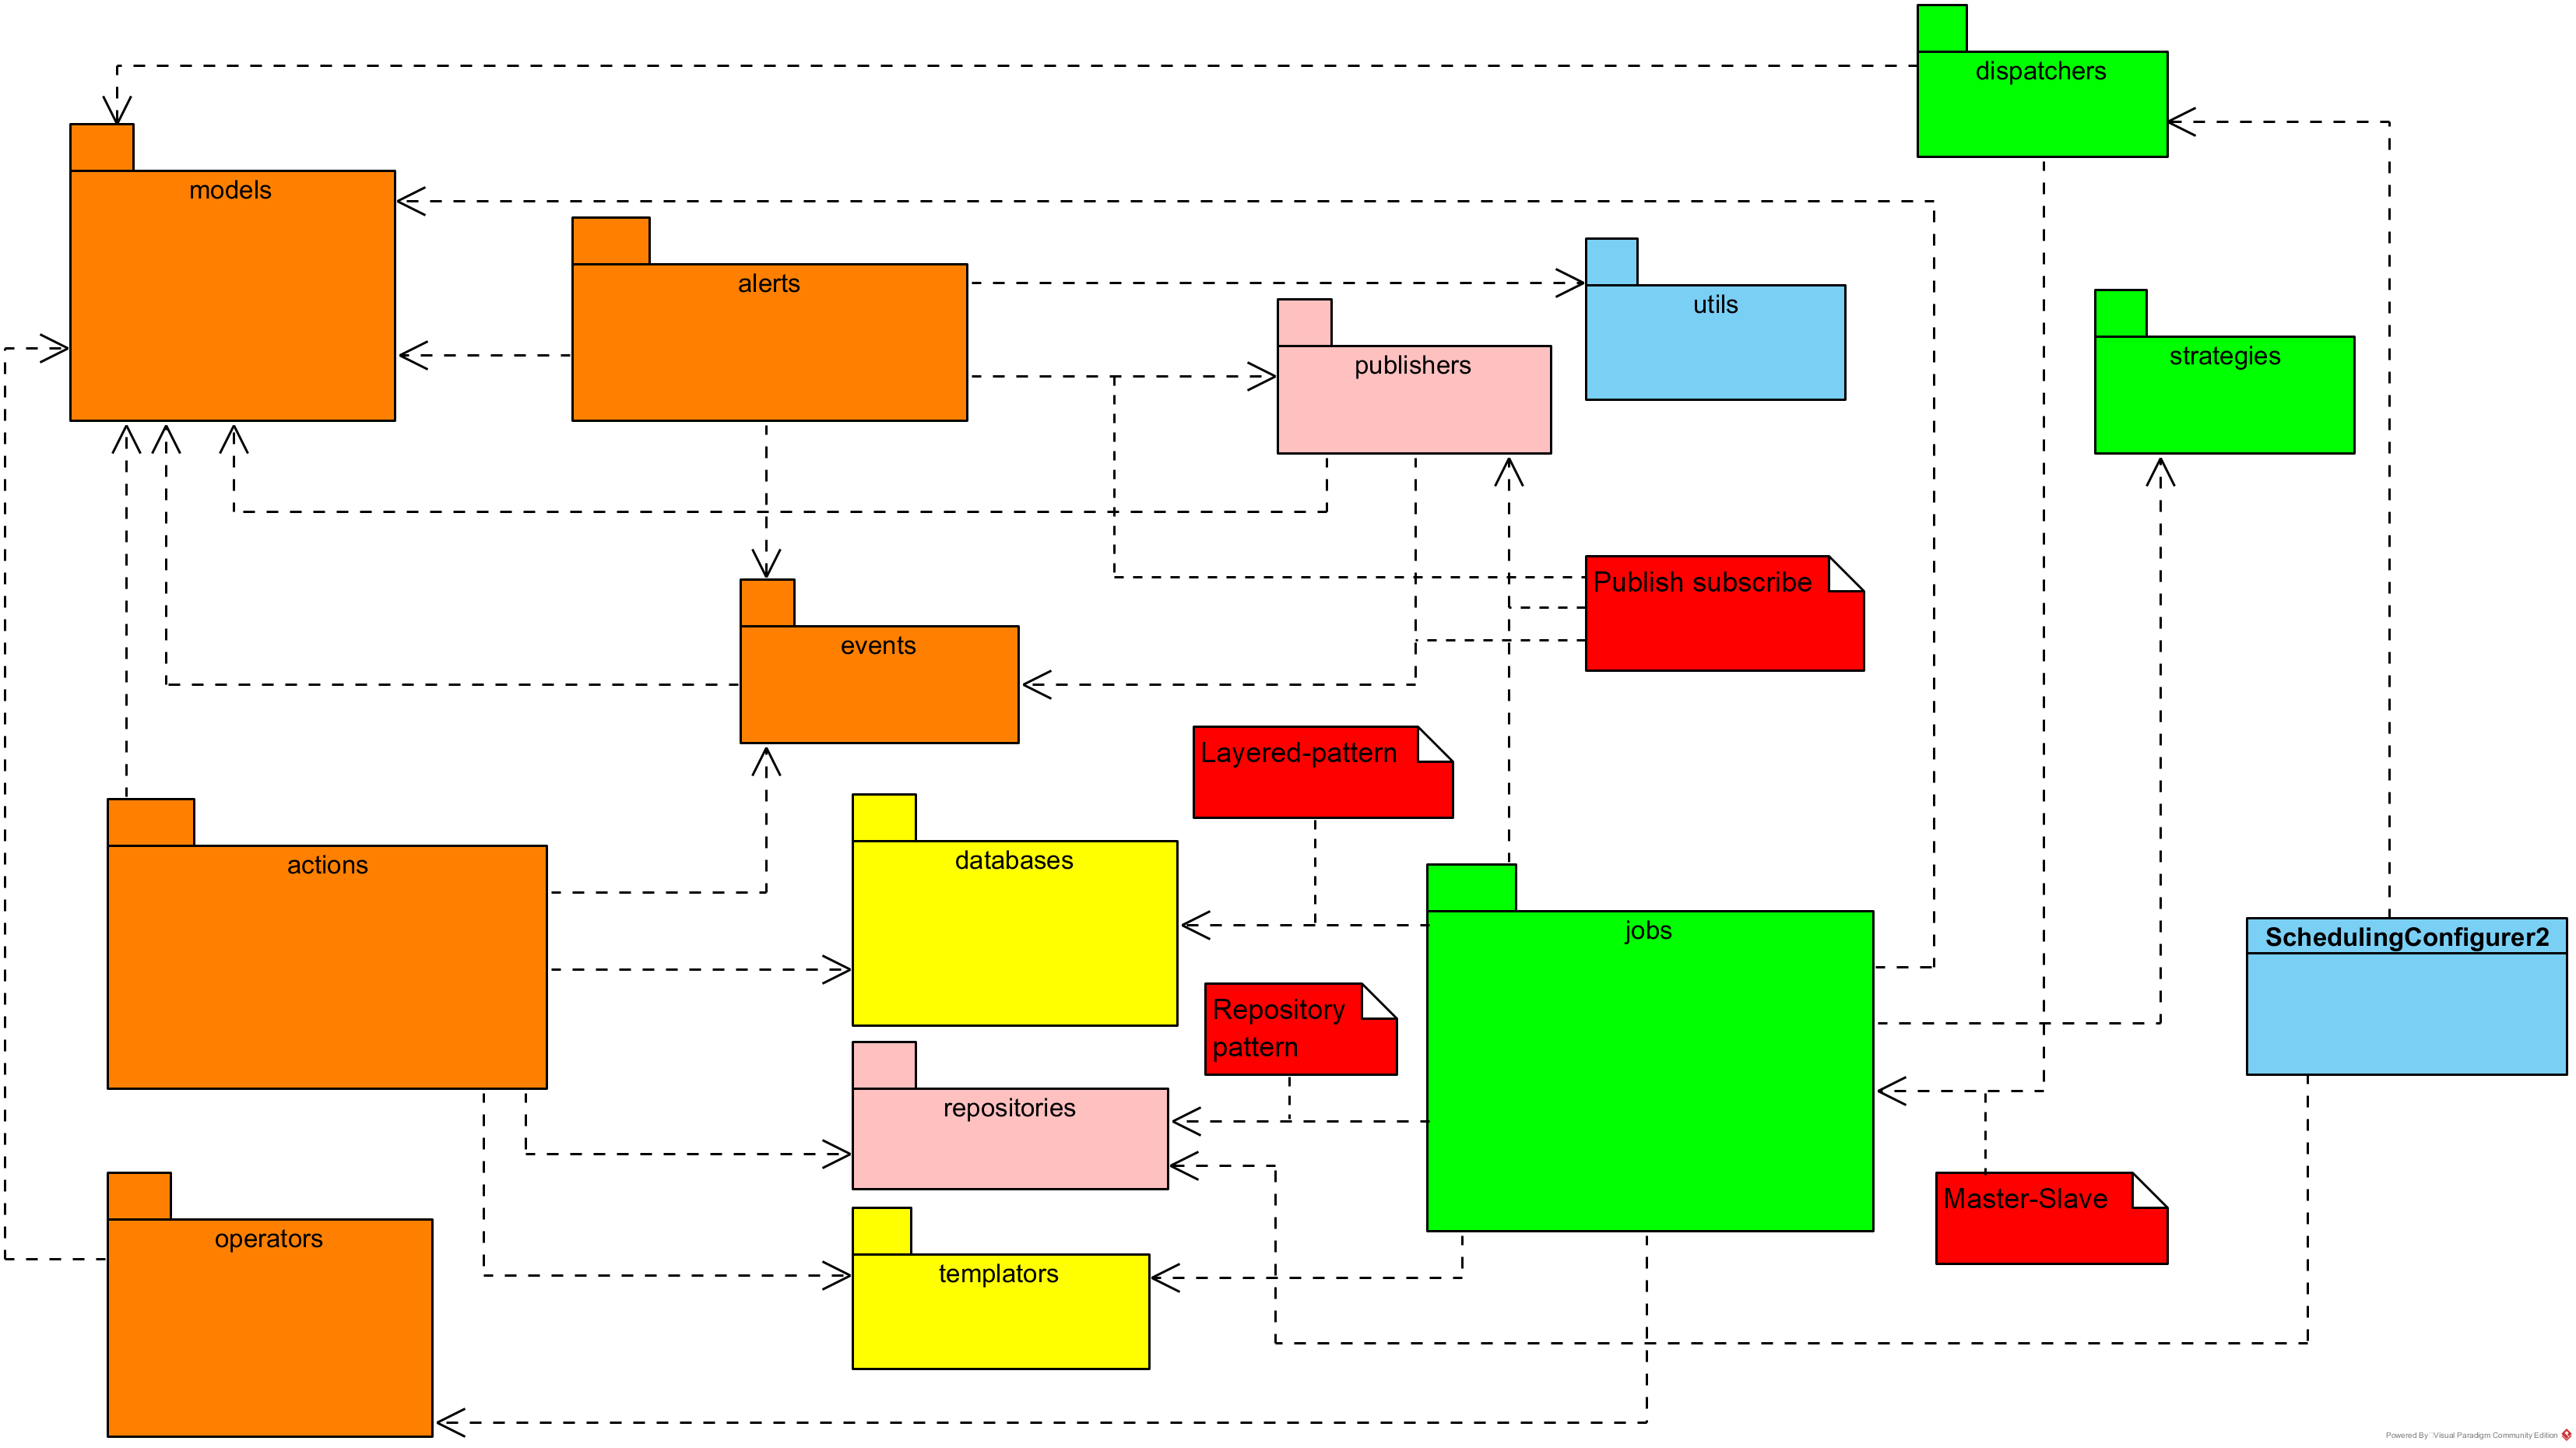
\includegraphics[width=1\linewidth]{./img/ArchitetturaGenerale.png}
	  	\caption{Architettura del prodotto \ProjectName{}}
	\end{figure}\\

\subsection{Classe SchedulingConfigurer}

		\begin{figure}[htbp]
           	\centering
       	    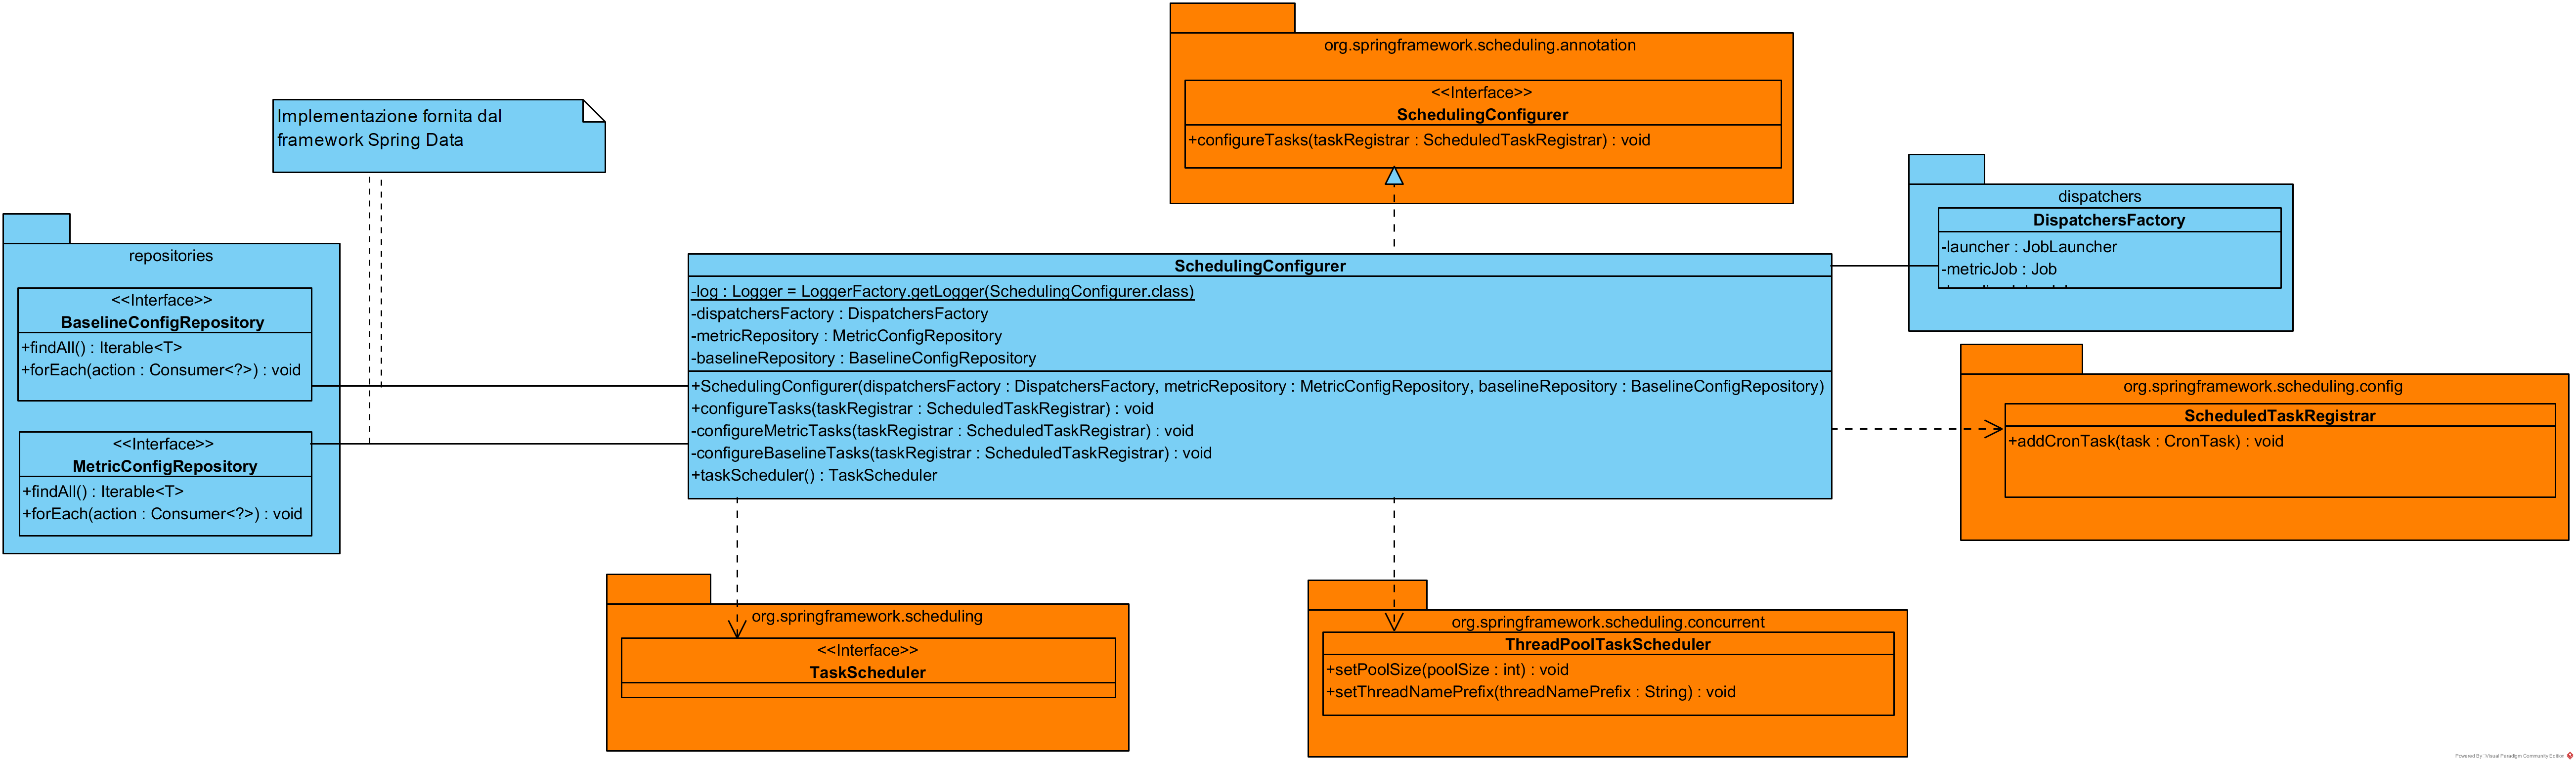
\includegraphics[width=\textwidth]{./img/DiagrammiClasse/SchedulingConfigurer.png}
   	        \caption[Diagramma della classe SchedulingConfigurer]{Diagramma della classe SchedulingConfigurer}
	    \end{figure}\\
        
        La classe SchedulingConfigurer si occupa di:
        \begin{itemize}
        	\item costruisce un oggetto \textit{DispatchersFactory} necessario per la costruzione di dispatchers;
        	\item costruisce un oggetto \textit{MetricConfigRepository} necessario per andare a prelevare da 
        		Elasticsearch la corretta configurazione per le metriche da creare;
        	\item costruisce un oggetto \textit{BaselineConfigRepository} necessario per andare a prelevare da 
        		Elasticsearch la corretta configurazione per le baseline da creare;
        	\item definire un oggetto \textit{TaskScheduler} necessario per la gestione dei task riguardanti
        		le metriche o le baseline all'interno dell'applicazione.
        \end{itemize}
        La classe implementa l'interfaccia \textit{SchedulerConfigurer} del framework Spring, documentata alla pagina
        \url{https://bit.ly/2IINkN8}. Questo perché permette di creare un oggetto \textit{TaskScheduler}
        capace di aggiungere operazioni alla coda delle operazioni da svolgere, la documentazione di questa 
        classe è presente all'indirizzo \url{https://bit.ly/2ksJbyi}. \\
        La classe utilizza le seguenti classi/interfacce:
        \begin{itemize}
        	\item \textbf{DispatchersFactory}: grazie a questa classe è possibile creare dispatchers che gestiscano la coda
        		dei processi;
        	\item \textbf{BaselineConfigRepositories}: permette di prelevare da Elasticsearch la configurazione prevista
        		per la costruzione di una baseline;
        	\item \textbf{MetricConfigRepositories}: permette di prelevare da Elasticsearch la configurazione prevista
        		per la costruzione di una metrica;
        	\item \textbf{TaskScheduler}: questa classe permette la programmazione di oggetti \textit{Runnables} in
        		base a diversi tipi di triggers;
        	\item \textbf{ThreadPoolTaskScheduler}: questa classe è l'implementazione dell'interfaccia \textit{TaskScheduler} 
				utilizzata in \ProjectName{};
        	\item \textbf{SchedulerTaskRegistrar}: è utilizzata come classe di supporto nella registrazione di 
        		operazioni nel \textit{TaskScheduler}.
        \end{itemize}
		
		
\subsection{Descrizione dei packages}

	\subsubsection{actions}
	
		\begin{figure}[H]
       		\centering
        	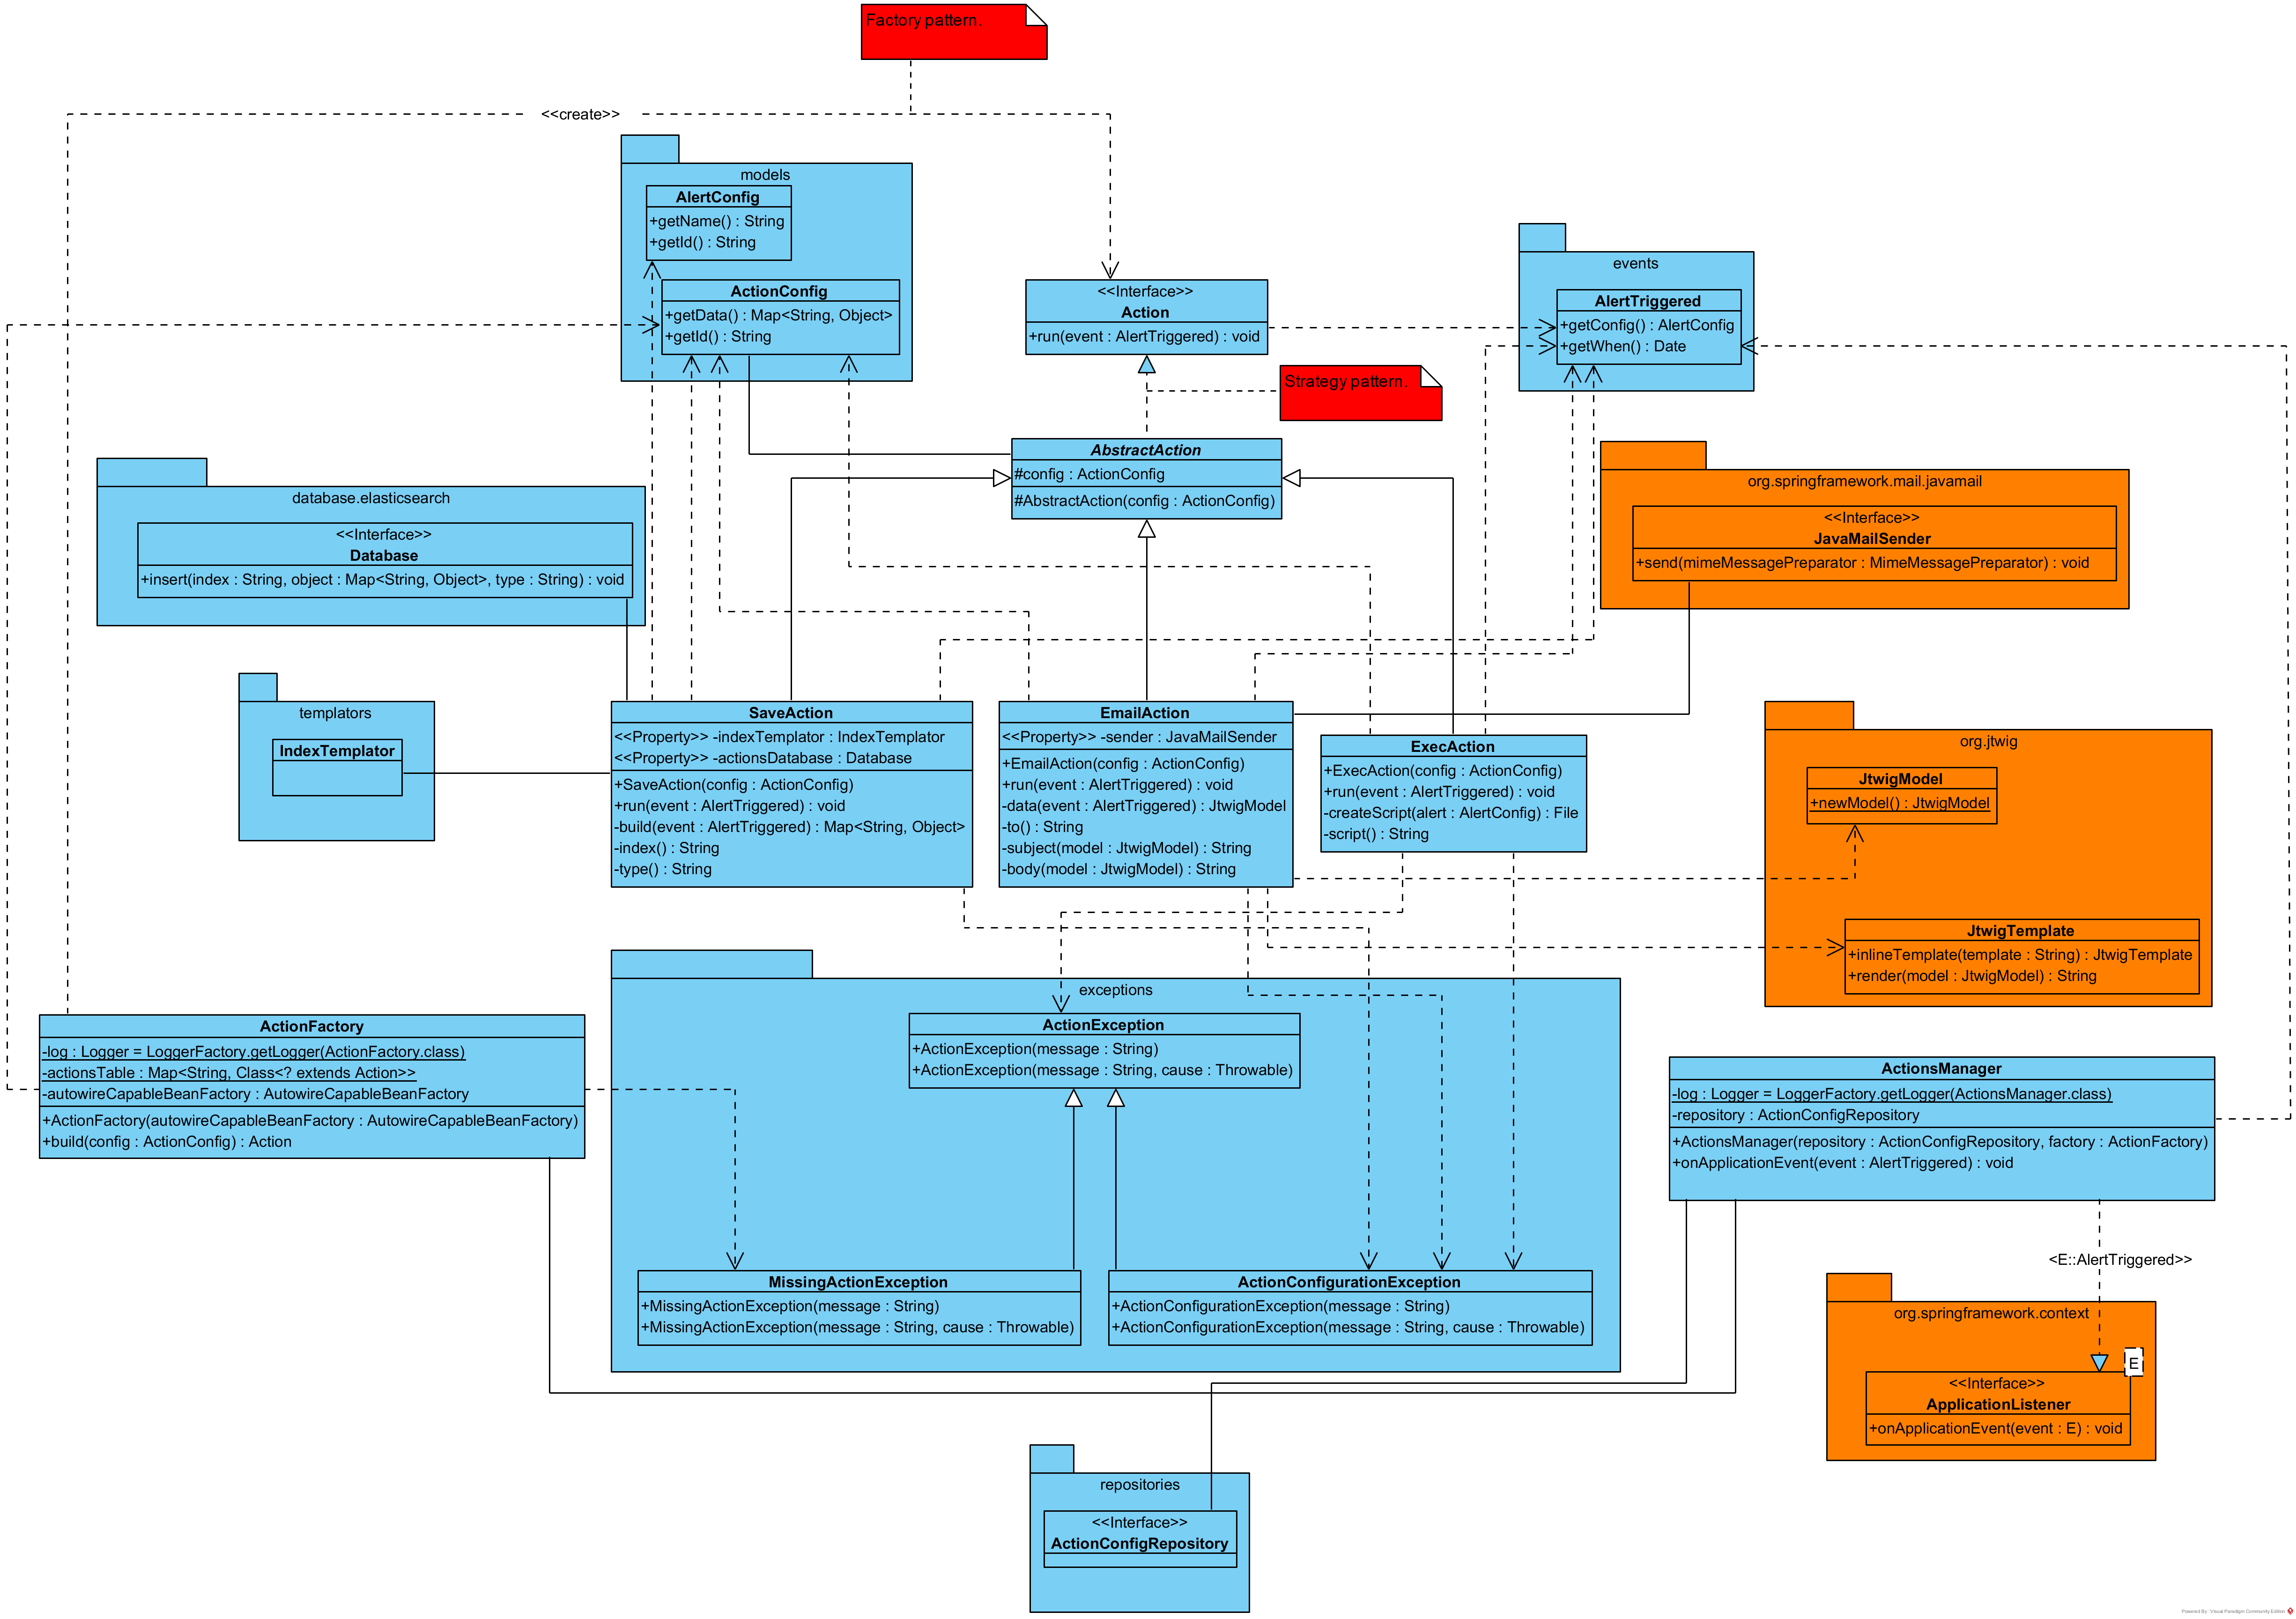
\includegraphics[width=\textwidth]{./img/DiagrammiClasse/actions.png}
        	\caption[Diagramma del package actions]{Diagramma del package actions}
       	\end{figure}\\

		\paragraph*{Descrizione}
			Questo package contiene tutte le classi inerenti alle azioni di rimedio, in 
			caso scatti un alert.\\
			Per aggiungerne di nuove approfondire in §\ref{newazione}.
		
		\paragraph*{Classi}
			\begin{itemize}
				\item \textbf{AbstractAction:} classe astratta di un'azione di rimedio, è già 
					presente il costruttore di default per un'azione di rimedio;
				\item \textbf{Action:} interfaccia per un'azione di rimedio; contiene il metodo \verb=run=
					che esegue l'azione di rimedio allo scattare dell'alert;
				\item \textbf{ActionFactory:} classe che permette di 
					costruire un azione in base ad una configurazione scelta;
				\item \textbf{ActionsManager:} gestore delle azioni di rimedio in caso scatti un alert;
				\item \textbf{EmailAction:} azione di rimedio che consiste nell'invio di un'email;
				\item \textbf{ExecAction:} azione di rimedio che consiste nell'esecuzione di un dato script;
				\item \textbf{SaveAction:} azione di rimedio che consiste nel salvare una ``alert notification''
					in un dato database.
			\end{itemize}\\
			
			Sottopackage \textbf{exceptions}:
			\begin{itemize}
				\item \textbf{ActionConfigurationException:} eccezione lanciata quando una configurazione
					per un'azione non è valida;
				\item \textbf{ActionException:} eccezione lanciata quando un'azione non può essere eseguita;
				\item \textbf{MissingActionException:} eccezione lanciata quando non è possibile definire 
					un'azione a causa di parametri in input non validi.
			\end{itemize}

\newpage

	\subsubsection{alerts}
	
		\begin{figure}[H]
			\centering
        	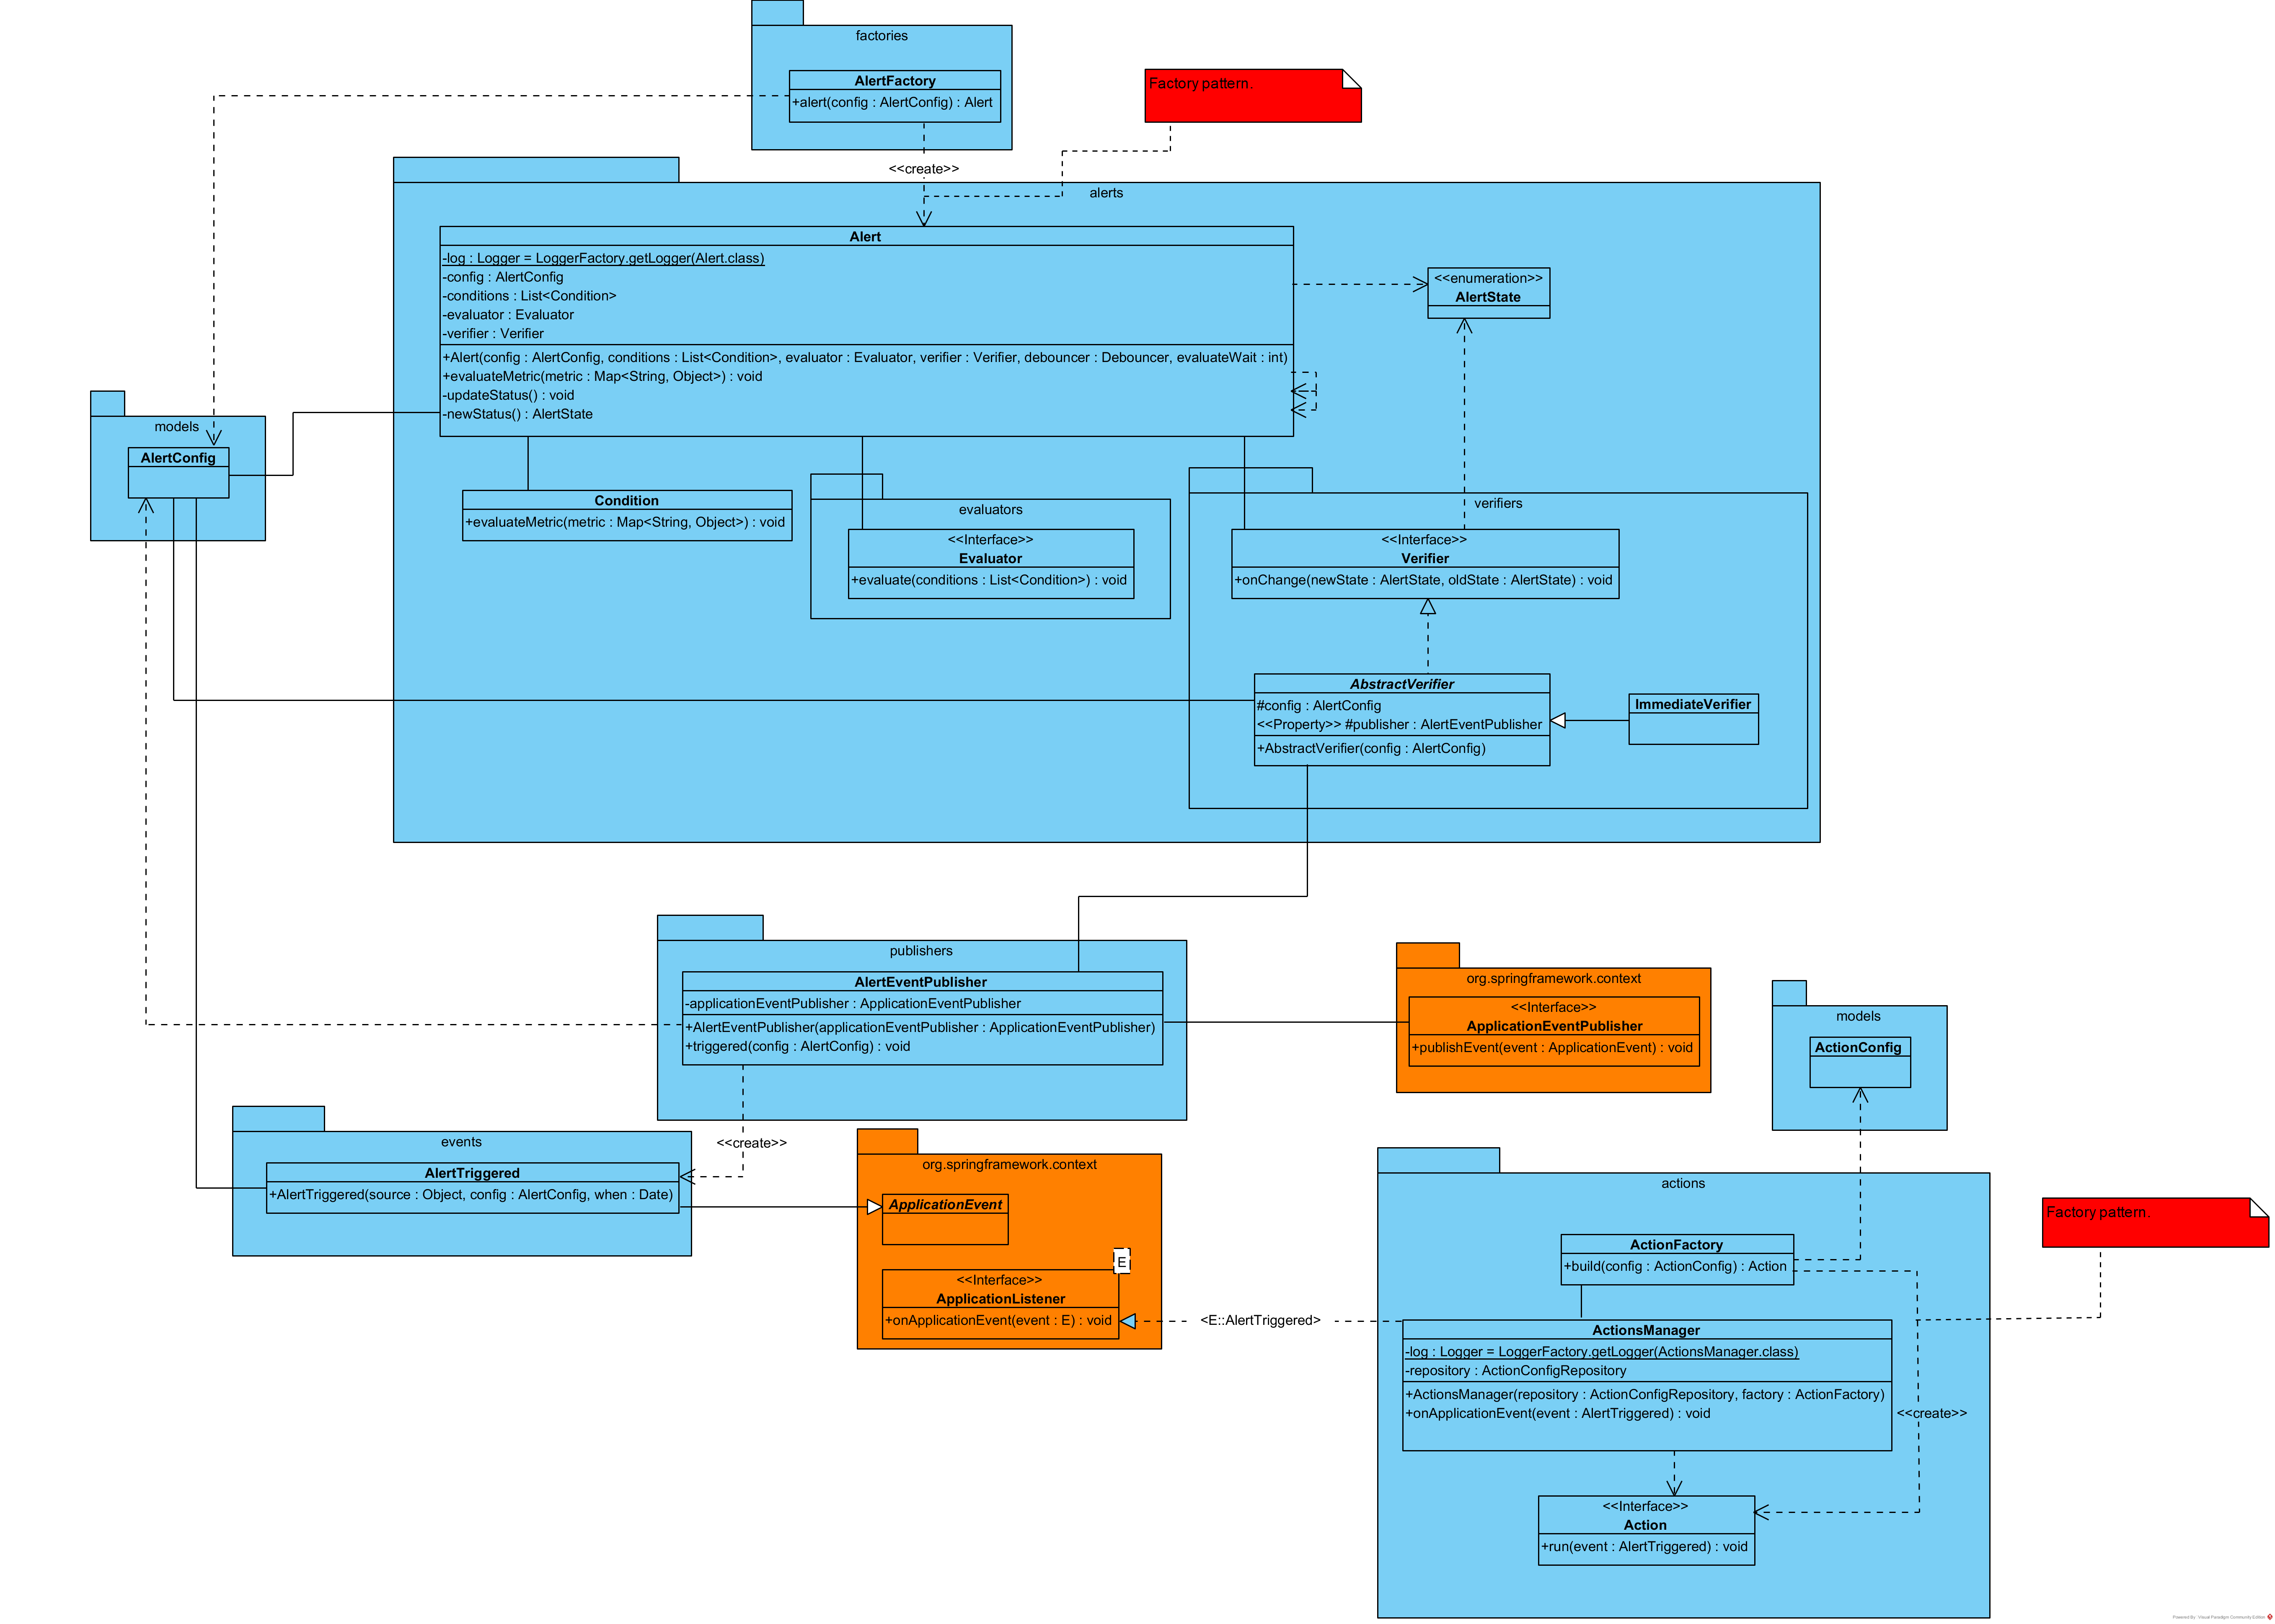
\includegraphics[width=\textwidth]{./img/DiagrammiClasse/alertToAction.png}
    	    \caption[Diagramma del package alerts]{Diagramma del package alerts ed interazione con il package actions}
		\end{figure}\\
       			
	    \begin{figure}[H]
    		\centering
        	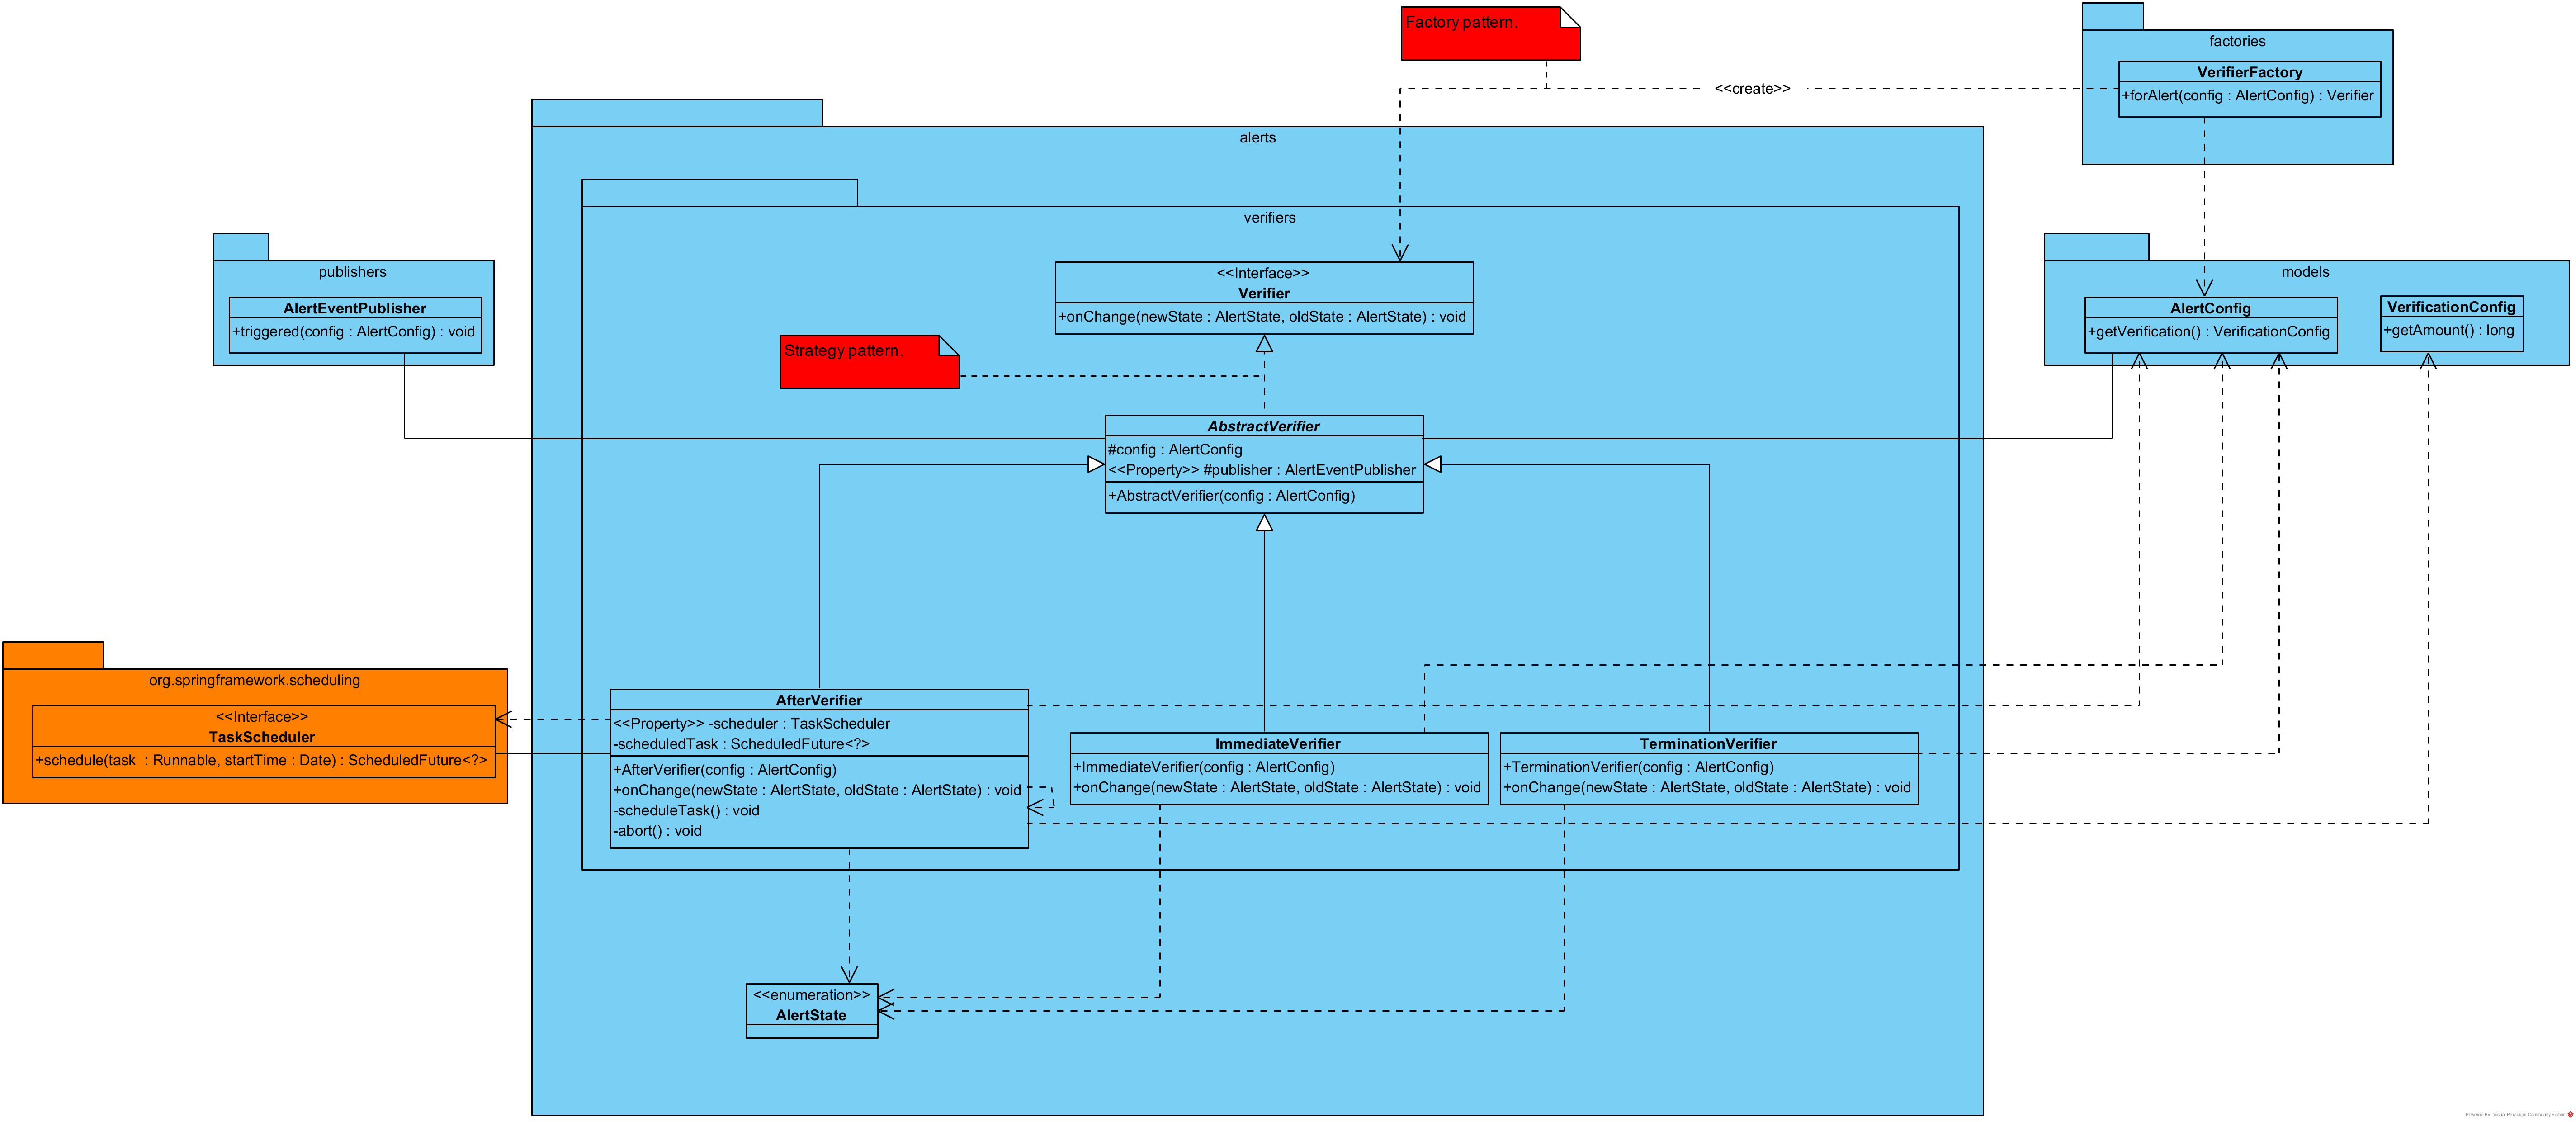
\includegraphics[width=\textwidth]{./img/DiagrammiClasse/verifiers.png}
    	    \caption[Diagramma del sottopackage verifiers]
	        {Diagramma del sottopackage verifiers del package alerts}
		\end{figure}\\
		
		\paragraph*{Descrizione}
			Questo package contiene le classi necessarie a descrivere lo scattare di un evento in cui
			è necessario fare un azione di rimedio per ovviare a possibili problemi.\\
			Per aggiungere nuovi valutatori o verificatori di alert è presente una guida in §\ref{newvalutatore}
			e §\ref{newverificatore}.
		
		\paragraph*{Classi}
			\begin{itemize}
				\item \textbf{Alert:} classe che descrive un alert, con una configurazione ed uno stato propri;
				\item \textbf{AlertsManager:} gestore degli alerts e controlla gli eventi alla creazione di una metrica; 
				\item \textbf{AlertState:} classe che descrive tutti i possibili stati di un alert;
				\item \textbf{BaselineRetriever:} classe che prende il valore di una baseline dato il tempo stimato;
				\item \textbf{Condition:} classe che descrive una condizione;
				\item \textbf{MetricState:} classe che descrive lo stato di una condizione sulle metriche,
					conserva l'ultima metrica e può filtrare le metriche in arrivo.
			\end{itemize}\\
			
			Sottopackage \textbf{evaluators}:
			\begin{itemize}
				\item \textbf{Evaluator:} interfaccia che descrive un valutatore di alerts;
				\item \textbf{AllMatchEvaluator:} valutatore che ritorna \verb=true= se tutte le condizioni 
					sono vere;
				\item \textbf{AnyMatchEvaluator:} valutatore che ritorna \verb=true= se almeno una condizione 
					è vera.
			\end{itemize}\\
				
			Sottopackage \textbf{verifiers}:
			\begin{itemize}
				\item \textbf{AbstractVerifier:} classe astratta per un verificatore;
				\item \textbf{AfterVerifier:} verificatore che lancia un'azione di rimedio dopo
					alcuni secondi il verificarsi del cambio di stato dell'alert;
				\item \textbf{ImmediateVerifier:} verificatore che lancia un'azione di rimedio non
					appena si verifica un cambio di stato dell'alert;
				\item \textbf{TerminationVerifier:} verificatore che lancia un'azione di rimedio 
					dopo che l'evento scatenante l'alert sia terminato;
				\item \textbf{Verifier:} interfaccia per un oggetto che riceve uno stato per un alert
					e decide se o quando lanciare un'azione di rimedio.
			\end{itemize}\\
			
			Sottopackage \textbf{factories}:\\
			\begin{itemize}
				\item \textbf{AlertFactory:} costruisce un alert data una configurazione;
				\item \textbf{EvaluatorFactory:} costruisce un valutatore data una configurazione;
				\item \textbf{VerifierFactory:} costruisce un verificatore data una configurazione.
			\end{itemize}
			
			Sottopackage \textbf{exceptions}:
			\begin{itemize}
				\item \textbf{BaselineNotFoundException:} eccezione lanciata quando non è possibile trovare 
					una baseline;
				\item \textbf{MissingEvaluatorException:} eccezione lanciata quando non è possibile definire 
					un valutatore a causa di parametri in input non validi;
				\item \textbf{MissingVerifierException:} eccezione lanciata quando non è possibile definire 
					un verificatore a causa di parametri in input non validi.
			\end{itemize}

\newpage
			
	\subsubsection{databases}


		\begin{figure}[H]
            	\centering
        	    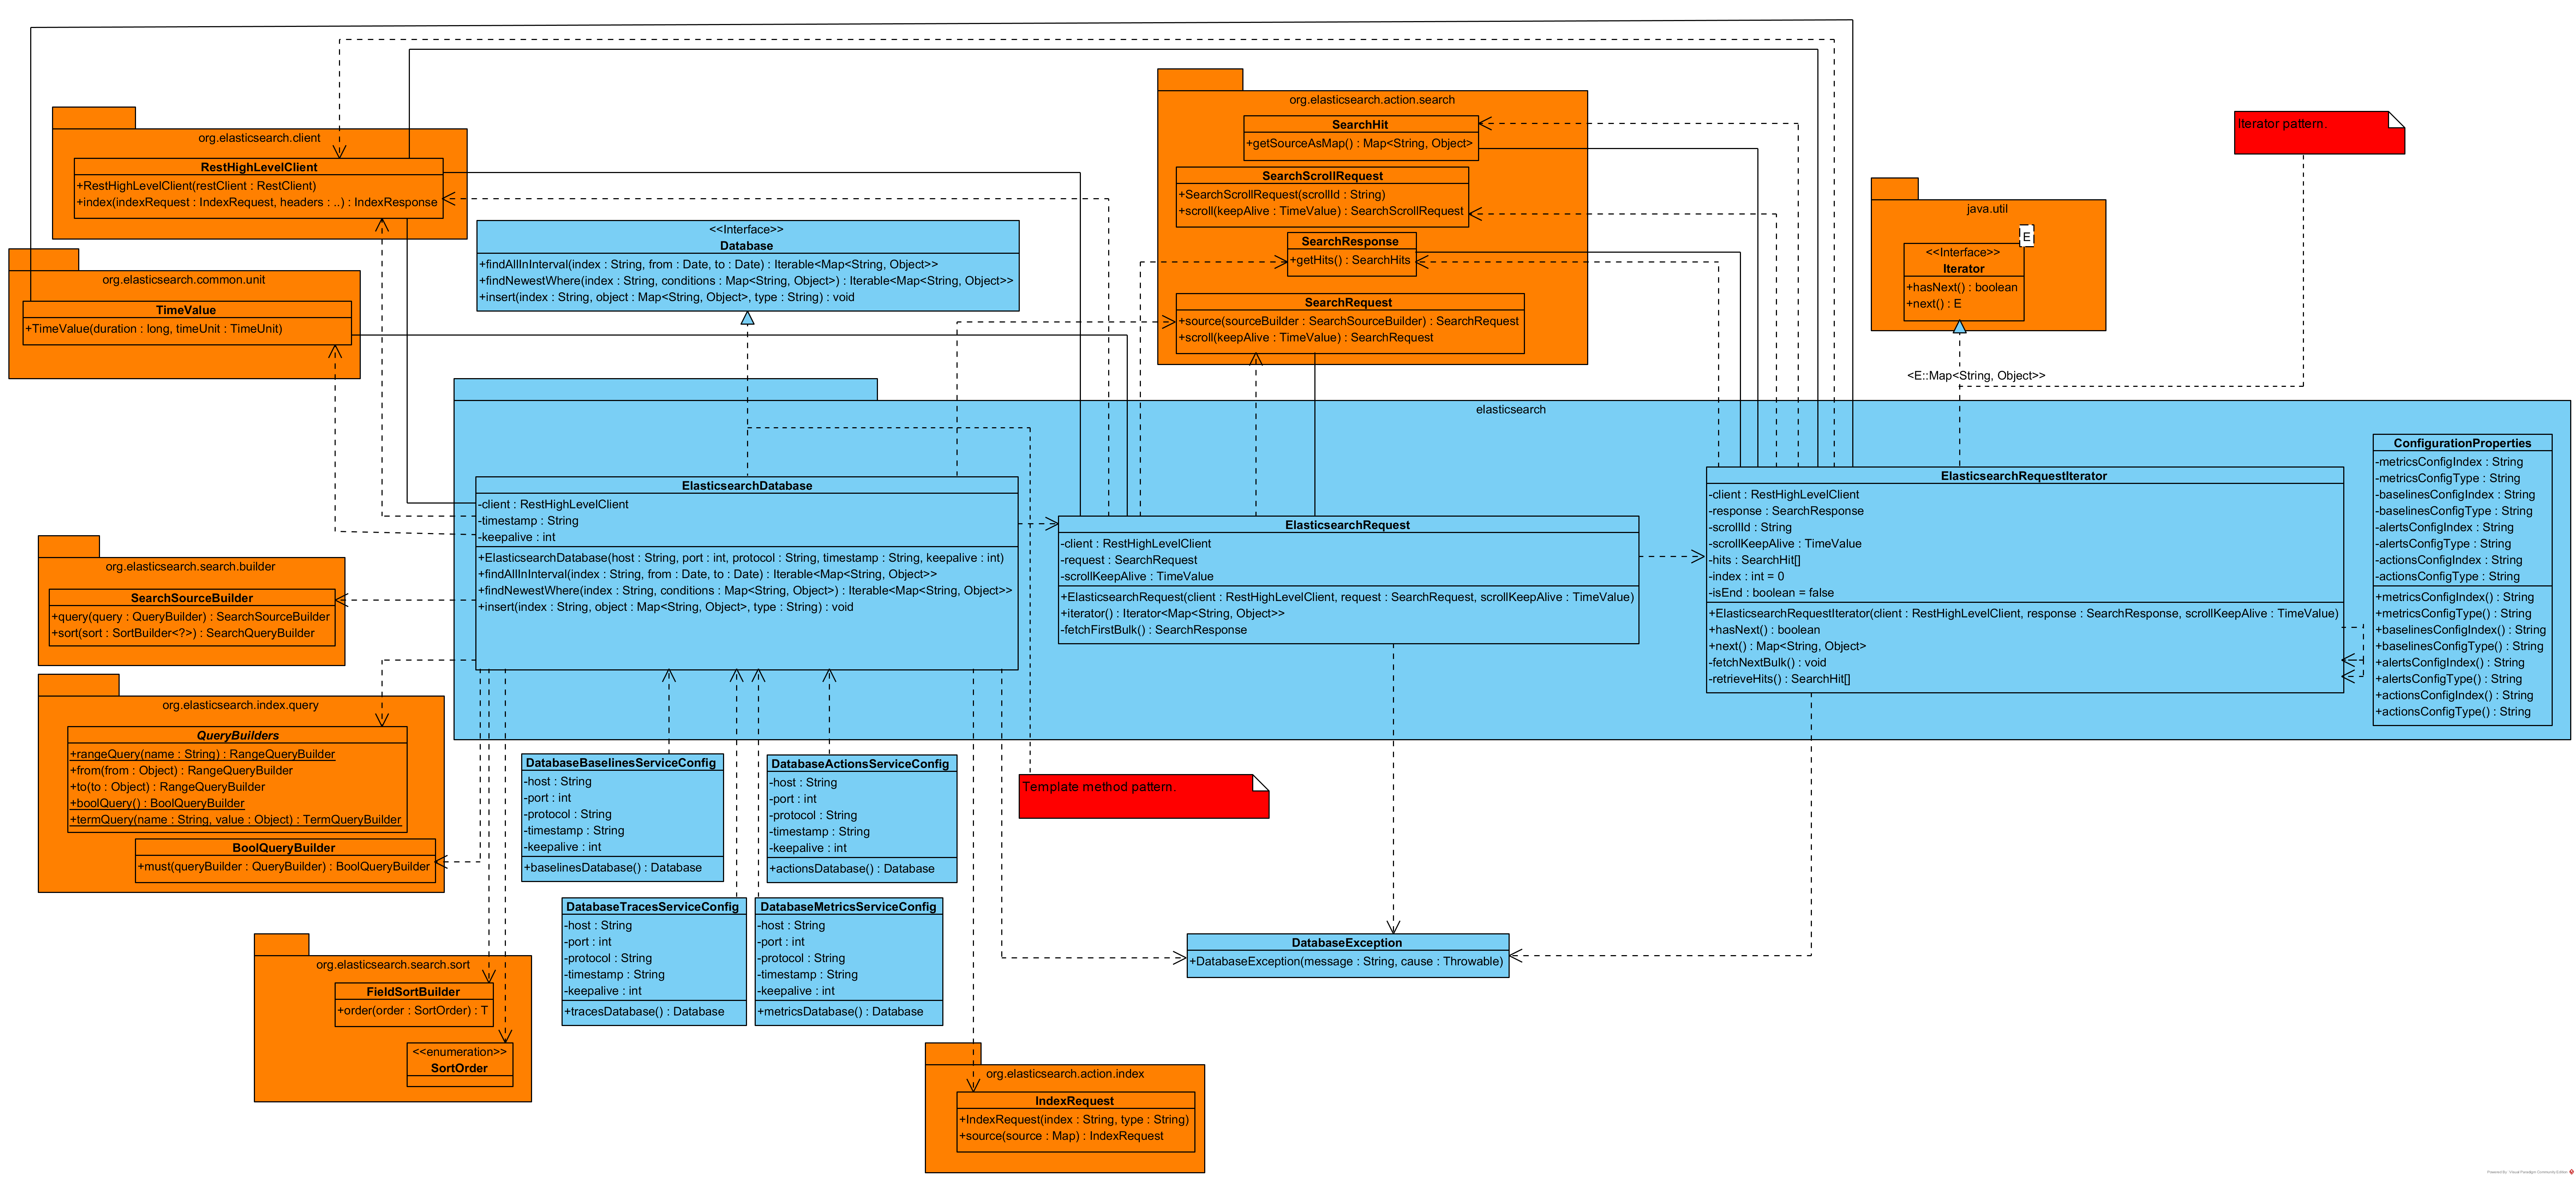
\includegraphics[width=\textwidth]{./img/DiagrammiClasse/databases.png}
        	    \caption[Diagramma del package databases]{Diagramma del package databases}
       	\end{figure}\\
		
		\paragraph*{Descrizione}
			Questo package contiene delle classi necessarie alla raccolta di dati utili nell'esecuzione.\\
			Per aggiungerne di nuovi vedere §\ref{newdatabase}.
			
			
		\paragraph*{Classi}
			
			\begin{itemize}
				\item \textbf{Database:} interfaccia che rappresenta un database astratto per la 
					raccolta dei dati;
				\item \textbf{DatabaseActionsServiceConfig:} classe che permette di creare un 
					database per la gestione delle azioni di rimedio;
				\item \textbf{DatabaseBaselinesServiceConfig:} classe che permette di creare un 
					database per la gestione delle baseline;
				\item \textbf{DatabaseMetricsServiceConfig:} classe che permette di creare un 
					database per la gestione delle metriche;
				\item \textbf{DatabaseException:} eccezione lanciata in caso di un'operazione 
					fallita nel database;
				\item \textbf{DatabaseTracesServiceConfig:} classe che permette di creare un 
					database per la gestione delle traces.
			\end{itemize}\\
			
			Sottopackage \textbf{elasticsearch}:
			\begin{itemize}
				\item \textbf{ElasticsearchDatabase:} implementazione della classe \verb=Database=
					per l'uso con Elasticsearch;
				\item \textbf{ElasticsearchRequest:} classe per effettuare le richieste ad Elasticsearch;
				\item \textbf{ElasticsearchRequestIterator:} iteratore per scorrere i risultati ottenuti
					da una richiesta al database Elasticsearch.
			\end{itemize}

\newpage

	\subsubsection{dispatchers}
	

		\begin{figure}[H]
           	\centering
            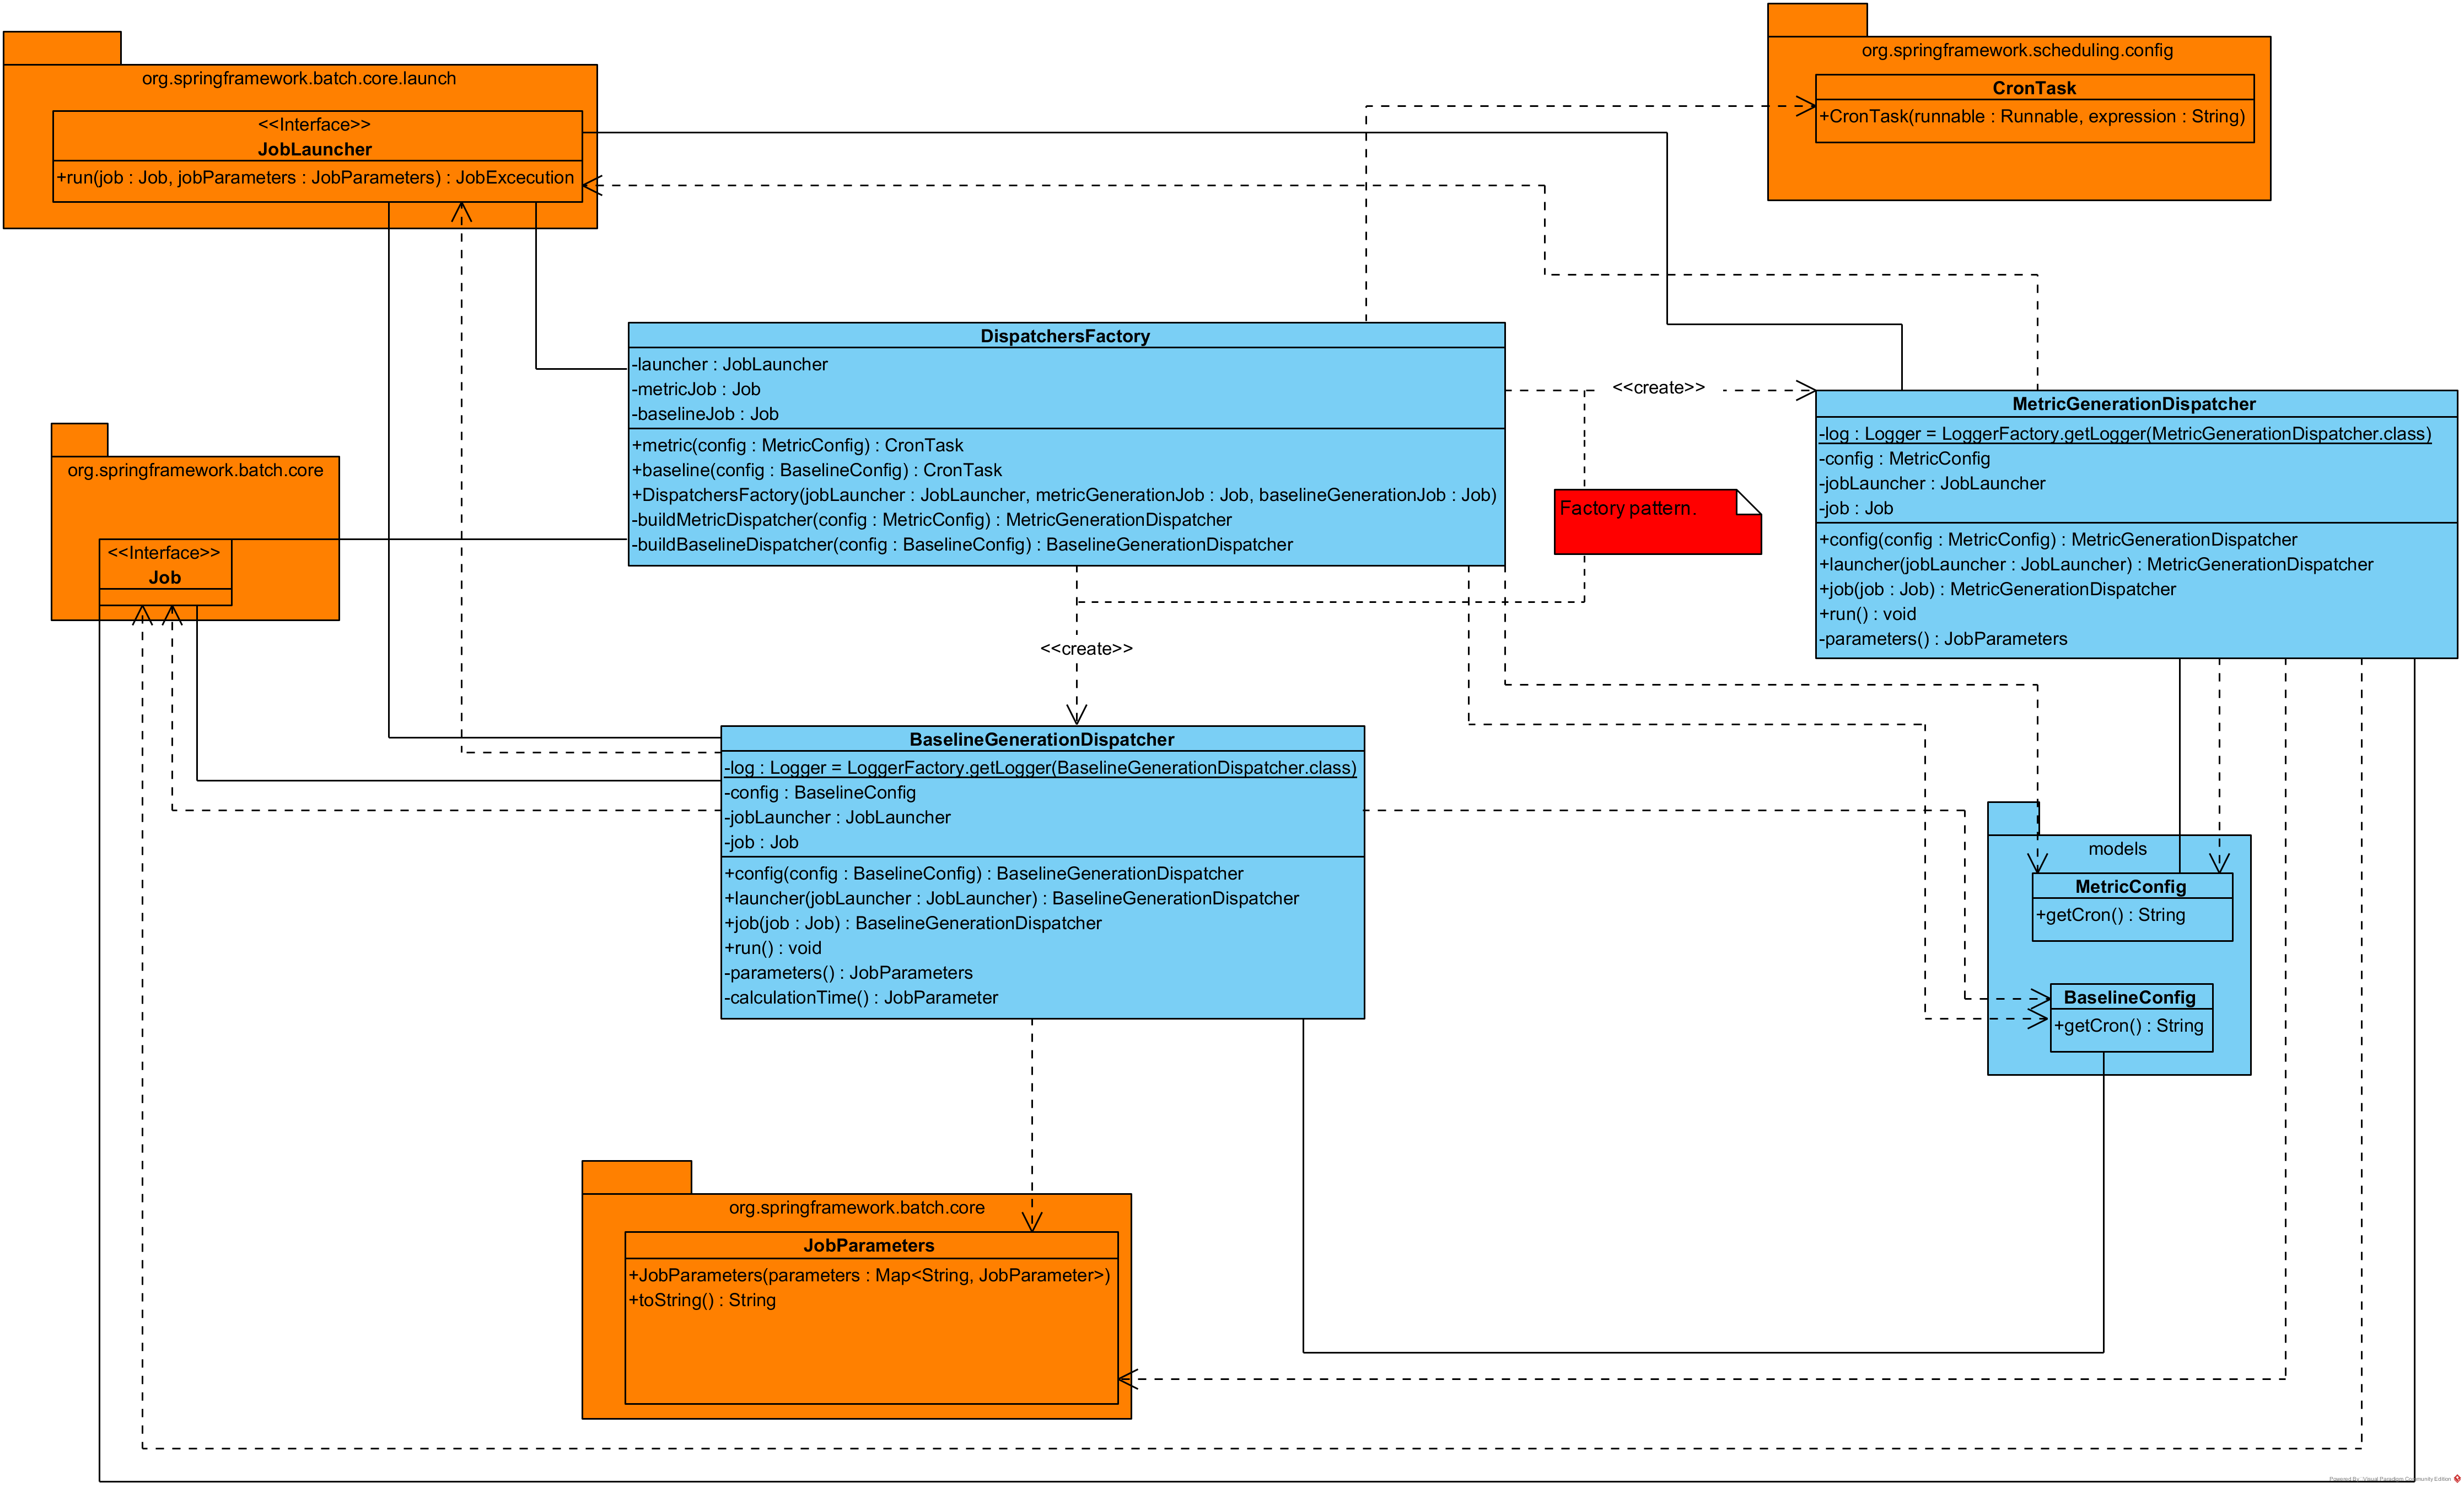
\includegraphics[width=\textwidth]{./img/DiagrammiClasse/dispatchers.png}
            \caption[Diagramma del package dispatchers]{Diagramma del package dispatchers}
       	\end{figure}\\
		
		\paragraph*{Descrizione}
			Questo package permette la creazione di dispachers per la richiesta di generazione di metriche e baseline.
		
		\paragraph*{Classi}
		\begin{itemize}
			\item \textbf{BaselineGenerationDispatcher:} rappresenta un dispacher per la generazione di baseline 
				basate sull'ultima ora;
			\item \textbf{MetricGenerationDispatcher:} rappresenta un dispacher per la generazione di metriche 
				basate sull'ora attuale;
			\item \textbf{DispatchersFactory:} classe che permette
				la creazione di dispachers in base alla configurazione scelta.
		\end{itemize}

\newpage

	\subsubsection{events}
		
		\paragraph*{Descrizione}
			Questo package contiene le classi che rappresentano il manifestarsi di un evento.
			
		\paragraph*{Classi}
			\begin{itemize}
				\item \textbf{AlertTriggered:} classe che rappresenta l'evento in cui è scattato
					un alert;
				\item \textbf{MetricCreated:} classe che rappresenta l'evento in cui è stata 
					creata una metrica.
			\end{itemize}	
			
	\subsubsection{jobs}
	
		\begin{figure}[H]
           	\centering
            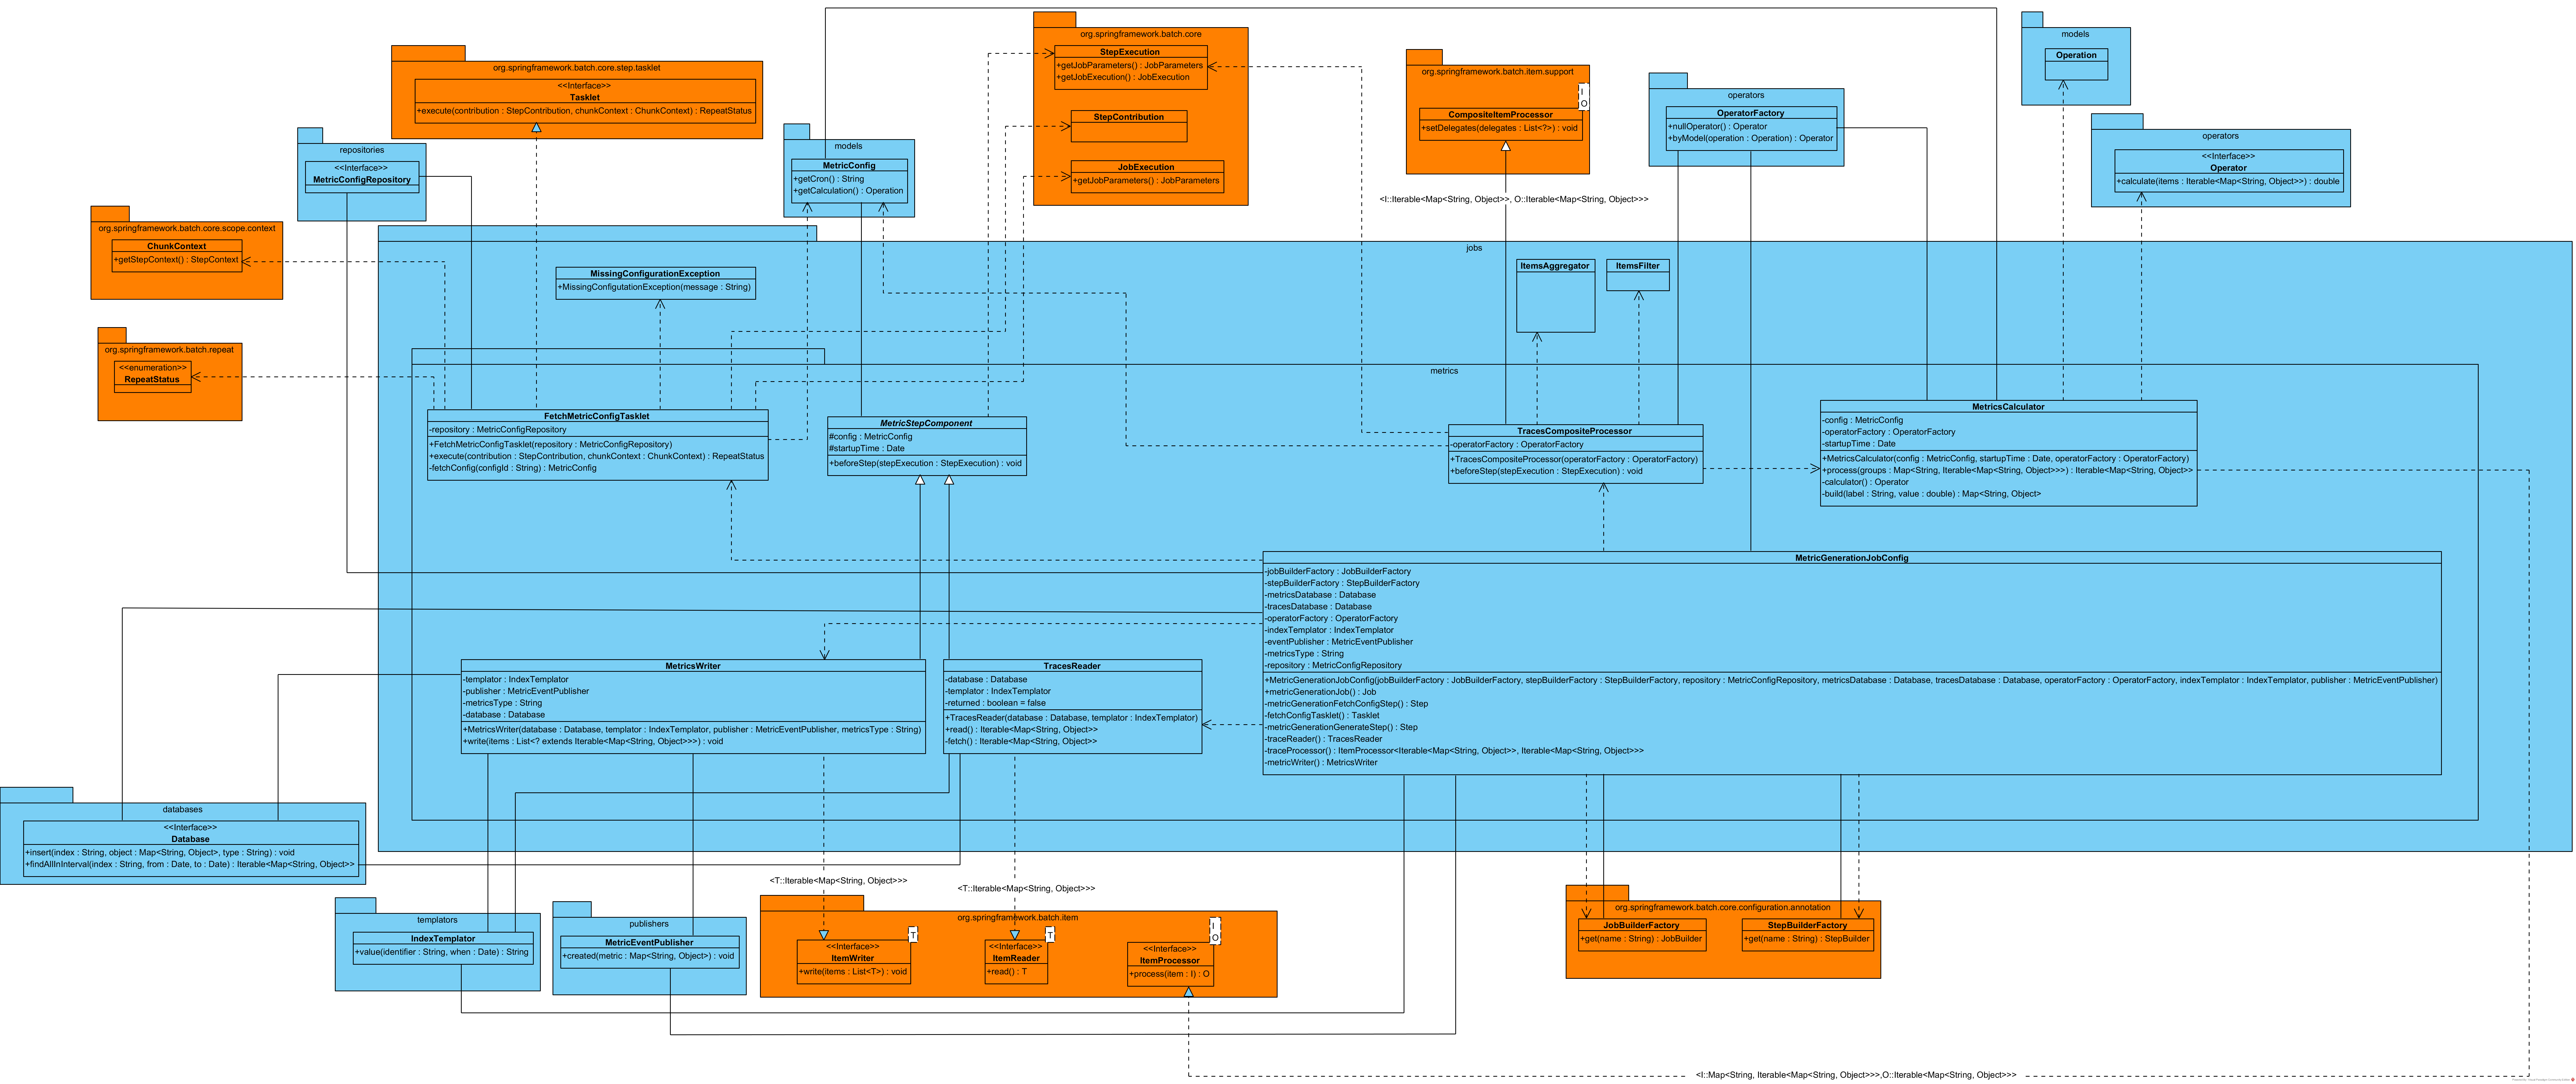
\includegraphics[width=\textwidth]{./img/DiagrammiClasse/metricJob.png}
            \caption[Diagramma del sottopackage metrics]
            {Diagramma del sottopackage metrics del package jobs (il sottopackage baseline è similare)}
       	\end{figure}
		
		\paragraph*{Descrizione}
			Questo package contiene le classi che rappresentano le operazioni che \ProjectName{}
			può svolgere.
		
		\paragraph*{Classi}
		
		\begin{itemize}
			\item \textbf{GroupItemsFilter:} classe che filtra tutti gli elementi di input suddivisi 
				in gruppi utilizzando una configurazione data;
			\item \textbf{ItemsAggregator:} classe che aggrega tutti gli input suddivisi in gruppi 
				in base ad una configurazione data;
			\item \textbf{ItemsFilter:} classe che filtra tutti gli input in base ad una configurazione
				data;
			\item \textbf{MissingConfigurationException:} eccezione che indica che il compito indicato in
				input non è presente nel database.			
		\end{itemize}\\
		
		Sottopackage \textbf{metrics}:
		\begin{itemize}
			\item \textbf{FetchMetricConfigTasklet:} classe per prelevare la configurazione della generazione
				delle metriche dal database;
			\item \textbf{MetricGenerationJobConfig:} configurazione per l'operazione di generazione di metriche
				da traces;
			\item \textbf{MetricsCalculator:} classe che calcola una metrica da ogni gruppo di traces in input;
			\item \textbf{MetricStepComponent:} classe astratta che recupera i parametri necessari dal contesto 
				del lavoro prima dell'esecuzione;
			\item \textbf{MetricsWriter:} classe che salva la metrica generata;
			\item \textbf{TracesCompositeProcessor:} definisce una serie di processori per generare una metrica
				da traces;
			\item \textbf{TracesReader:} classe per leggere le traces dal database.
		\end{itemize}\\
		
		Sottopackage \textbf{baselines}:
		\begin{itemize}
			\item \textbf{BaselineGenerationJobConfig:} configurazione per generare una baseline da delle metriche;
			\item \textbf{BaselinesCalculator:} calcola una baseline per ogni insieme di metriche in input;
			\item \textbf{BaselineStepComponent:} classe astratta che recupera i parametri necessari dal contesto 
				del lavoro prima dell'esecuzione;
			\item \textbf{BaselinesWriter:} classe che salva la baseline generata;
			\item \textbf{FetchBaselineConfigTasklet:} classe per prelevare la configurazione della generazione
				della baseline dal database;
			\item \textbf{MetricsCompositeProcessor:} definisce una serie di processori per generare una baseline
				da metriche;
			\item \textbf{MetricsGroupsAggregator:} aggrega tutti gli insiemi di metriche in gruppi;
			\item \textbf{MetricsReader:} classe per leggere metriche dal database.
		\end{itemize}

\newpage

	\subsubsection{models}
		
		\paragraph*{Descrizione}
			Questo package contiene tutte le configurazioni per le componenti del progetto.		
		
		\paragraph*{Classi}
		
		\begin{itemize}
			\item \textbf{ActionConfig:} configurazione per un'azione di rimedio;
			\item \textbf{AlertConfig:} configurazione per un alert;
			\item \textbf{BaselineConfig:} configurazione per una baseline;
			\item \textbf{BaselineValue:} configurazione per un valore prelevato da una baseline;
			\item \textbf{ConditionConfig:} configurazione per una condizione;
			\item \textbf{MetricConfig:} configurazione per una metrica;
			\item \textbf{Operation:} operazione generica da salvare nel database;
			\item \textbf{VerificationConfig:} configurazione per un verificatore di eventi.
		\end{itemize}
		
		Sottopackage \textbf{contracts}:
		\begin{itemize}
			\item \textbf{AggregableConfig:} modello di configurazione che permette di aggregare elementi
				dato un \verb=Operator=;			
			\item \textbf{FilterableConfig:} modello di configurazione che permette di filtrare elementi
				dato un insieme di \verb=Operator=;	
		\end{itemize}

\newpage
		
	\subsubsection{operators}
	
		\begin{figure}[H]
           	\centering
            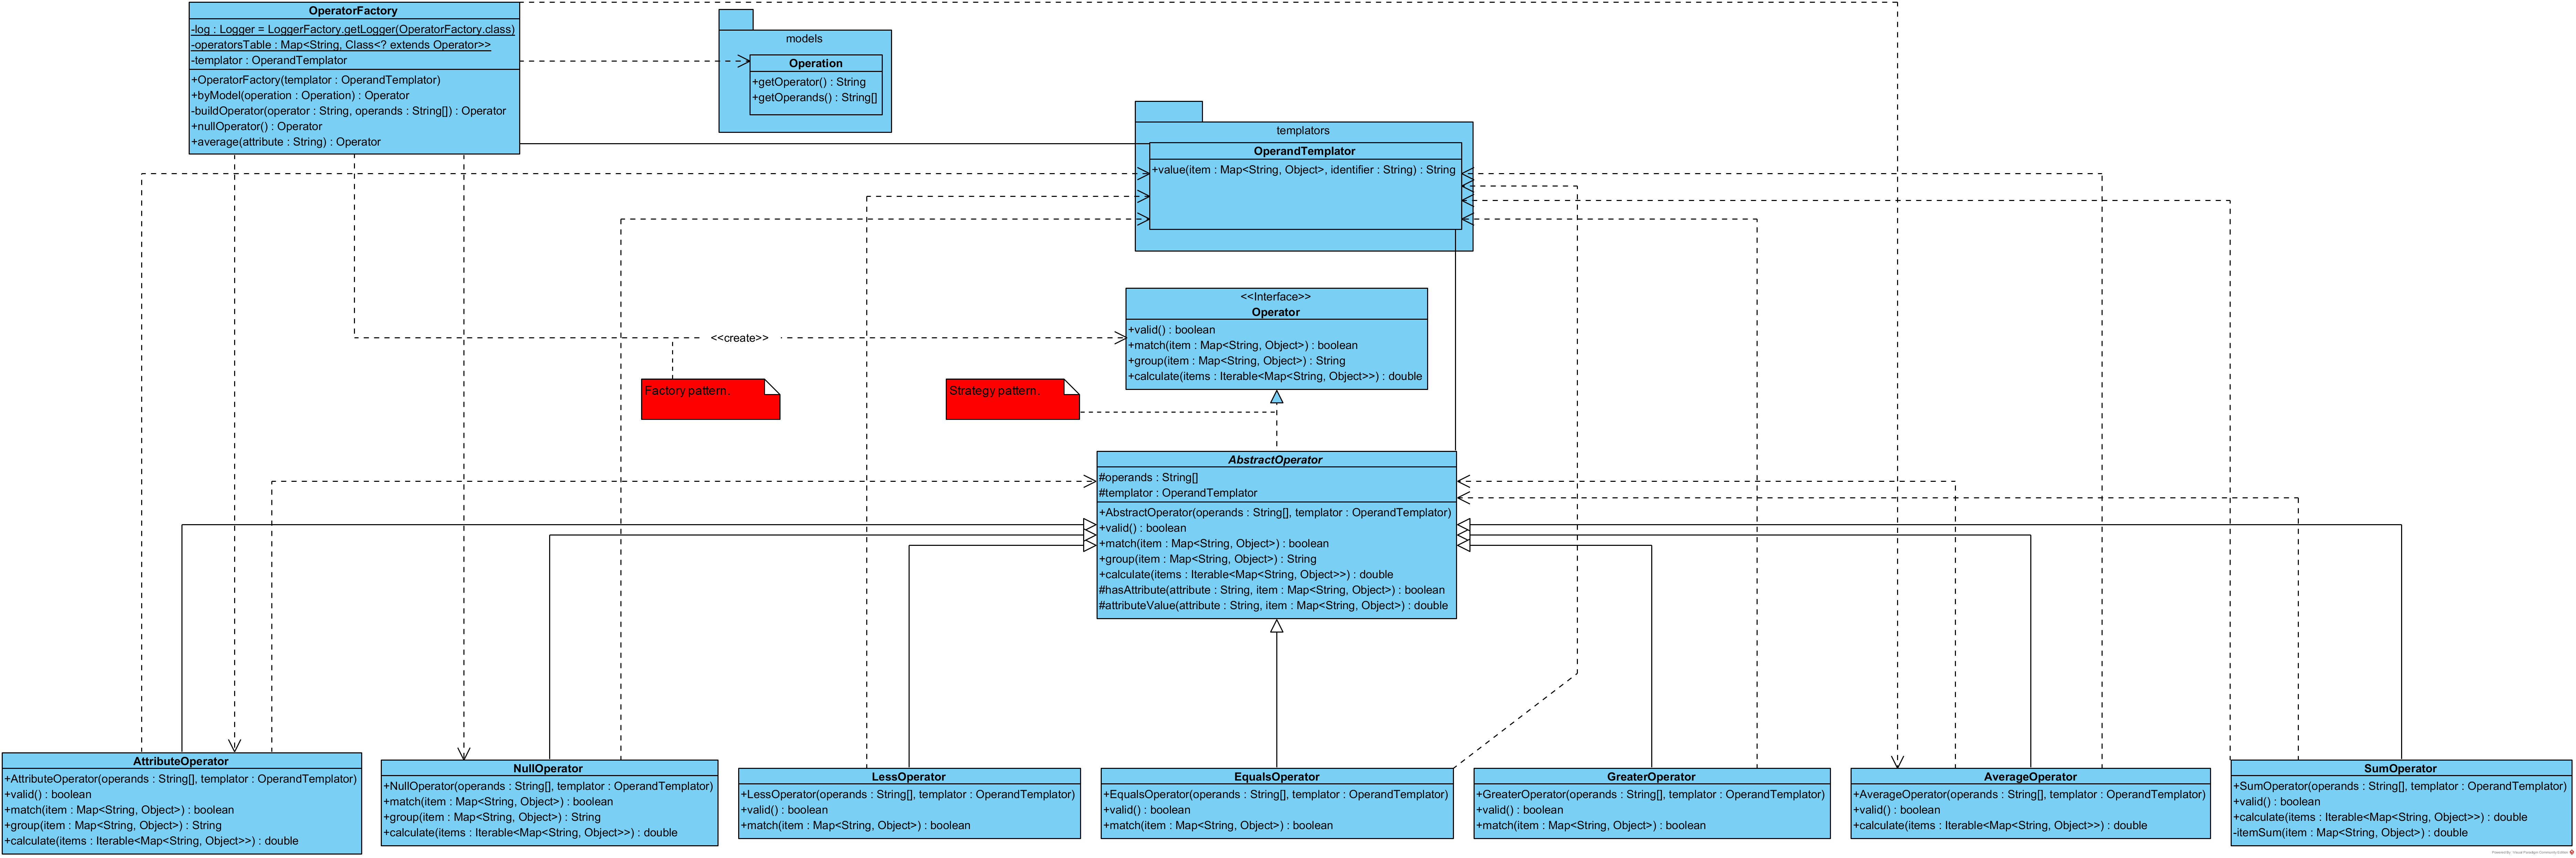
\includegraphics[width=\textwidth]{./img/DiagrammiClasse/operators.png}
            \caption[Diagramma del package operators]{Diagramma del package operators}
       	\end{figure}
		
		\paragraph*{Descrizione}
			Questo package raccoglie tutti gli operatori coinvolti nei diversi calcoli presenti in
			\ProjectName{}.\\
			Per aggiungerne di nuovi vedere §\ref{newoperatore}.
			
		\paragraph*{Classi}
		\begin{itemize}	
			\item \textbf{AbstractOperator:} classe astratta con un'implementazione base di un operatore;
			\item \textbf{AttributeOperator:} operatore per ottenere l'attributo di un oggetto;
			\item \textbf{AverageOperator:} operatore per calcolare la media di un attributo in un 
				insieme di traces;
			\item \textbf{EqualsOperator:} operatore per verificare che due valori siano uguali;
			\item \textbf{GreaterOperator:} operatore per verificare che il primo operatore sia maggiore 
				del secondo;
			\item \textbf{LessOperator:}operatore per verificare che il primo operatore sia minore 
				del secondo;
			\item \textbf{NullOperator:} operatore nullo che non effettua nessuna operazione o calcolo;
			\item \textbf{Operator:} interfaccia per operatori in grado di eseguire operazioni su oggetti;
			\item \textbf{OperatorFactory:} classe che  permette di 	
				costruire un operatore in base ad una configurazione scelta;
			\item \textbf{SumOperator:} operatore che effettua la somma di un attributo in un insieme di oggetti.
		\end{itemize}

\newpage
		
	\subsubsection{publishers}
		
		\paragraph*{Descrizione}
			Questo package contiene le classi responsabili della notifica dell'avvenimento di un evento.
		
		\paragraph*{Classi}
		
		\begin{itemize}
			\item \textbf{AlertEventPublisher:} notifica per eventi riguardanti gli alerts;
			\item \textbf{MetricEventPublisher:} notifica per eventi riguardanti le metriche come,
				ad esempio, la creazione di una di queste.
		\end{itemize}
		
	\subsubsection{repositories}
		
		\paragraph*{Descrizione}
			In questo package sono contenute le classi necessarie per prelevare le configurazioni
			degli oggetti da Elasticsearch.
		
		\paragraph*{Classi}
			
			\begin{itemize}
				\item \textbf{ActionConfigRepository:} repository per prelevare un \verb=ActionConfig= 
					da Elasticsearch;
				\item \textbf{AlertConfigRepository:} repository per prelevare un \verb=AlertConfig= 
					da Elasticsearch;
				\item \textbf{BaselineConfigRepository:} repository per prelevare un \verb=BaselineConfig= 
					da Elasticsearch;
				\item \textbf{MetricConfigRepository:} repository per prelevare un \verb=MetricConfig= 
					da Elasticsearch.
			\end{itemize}

\newpage

	\subsubsection{strategies}
	

		\begin{figure}[H]
           	\centering
            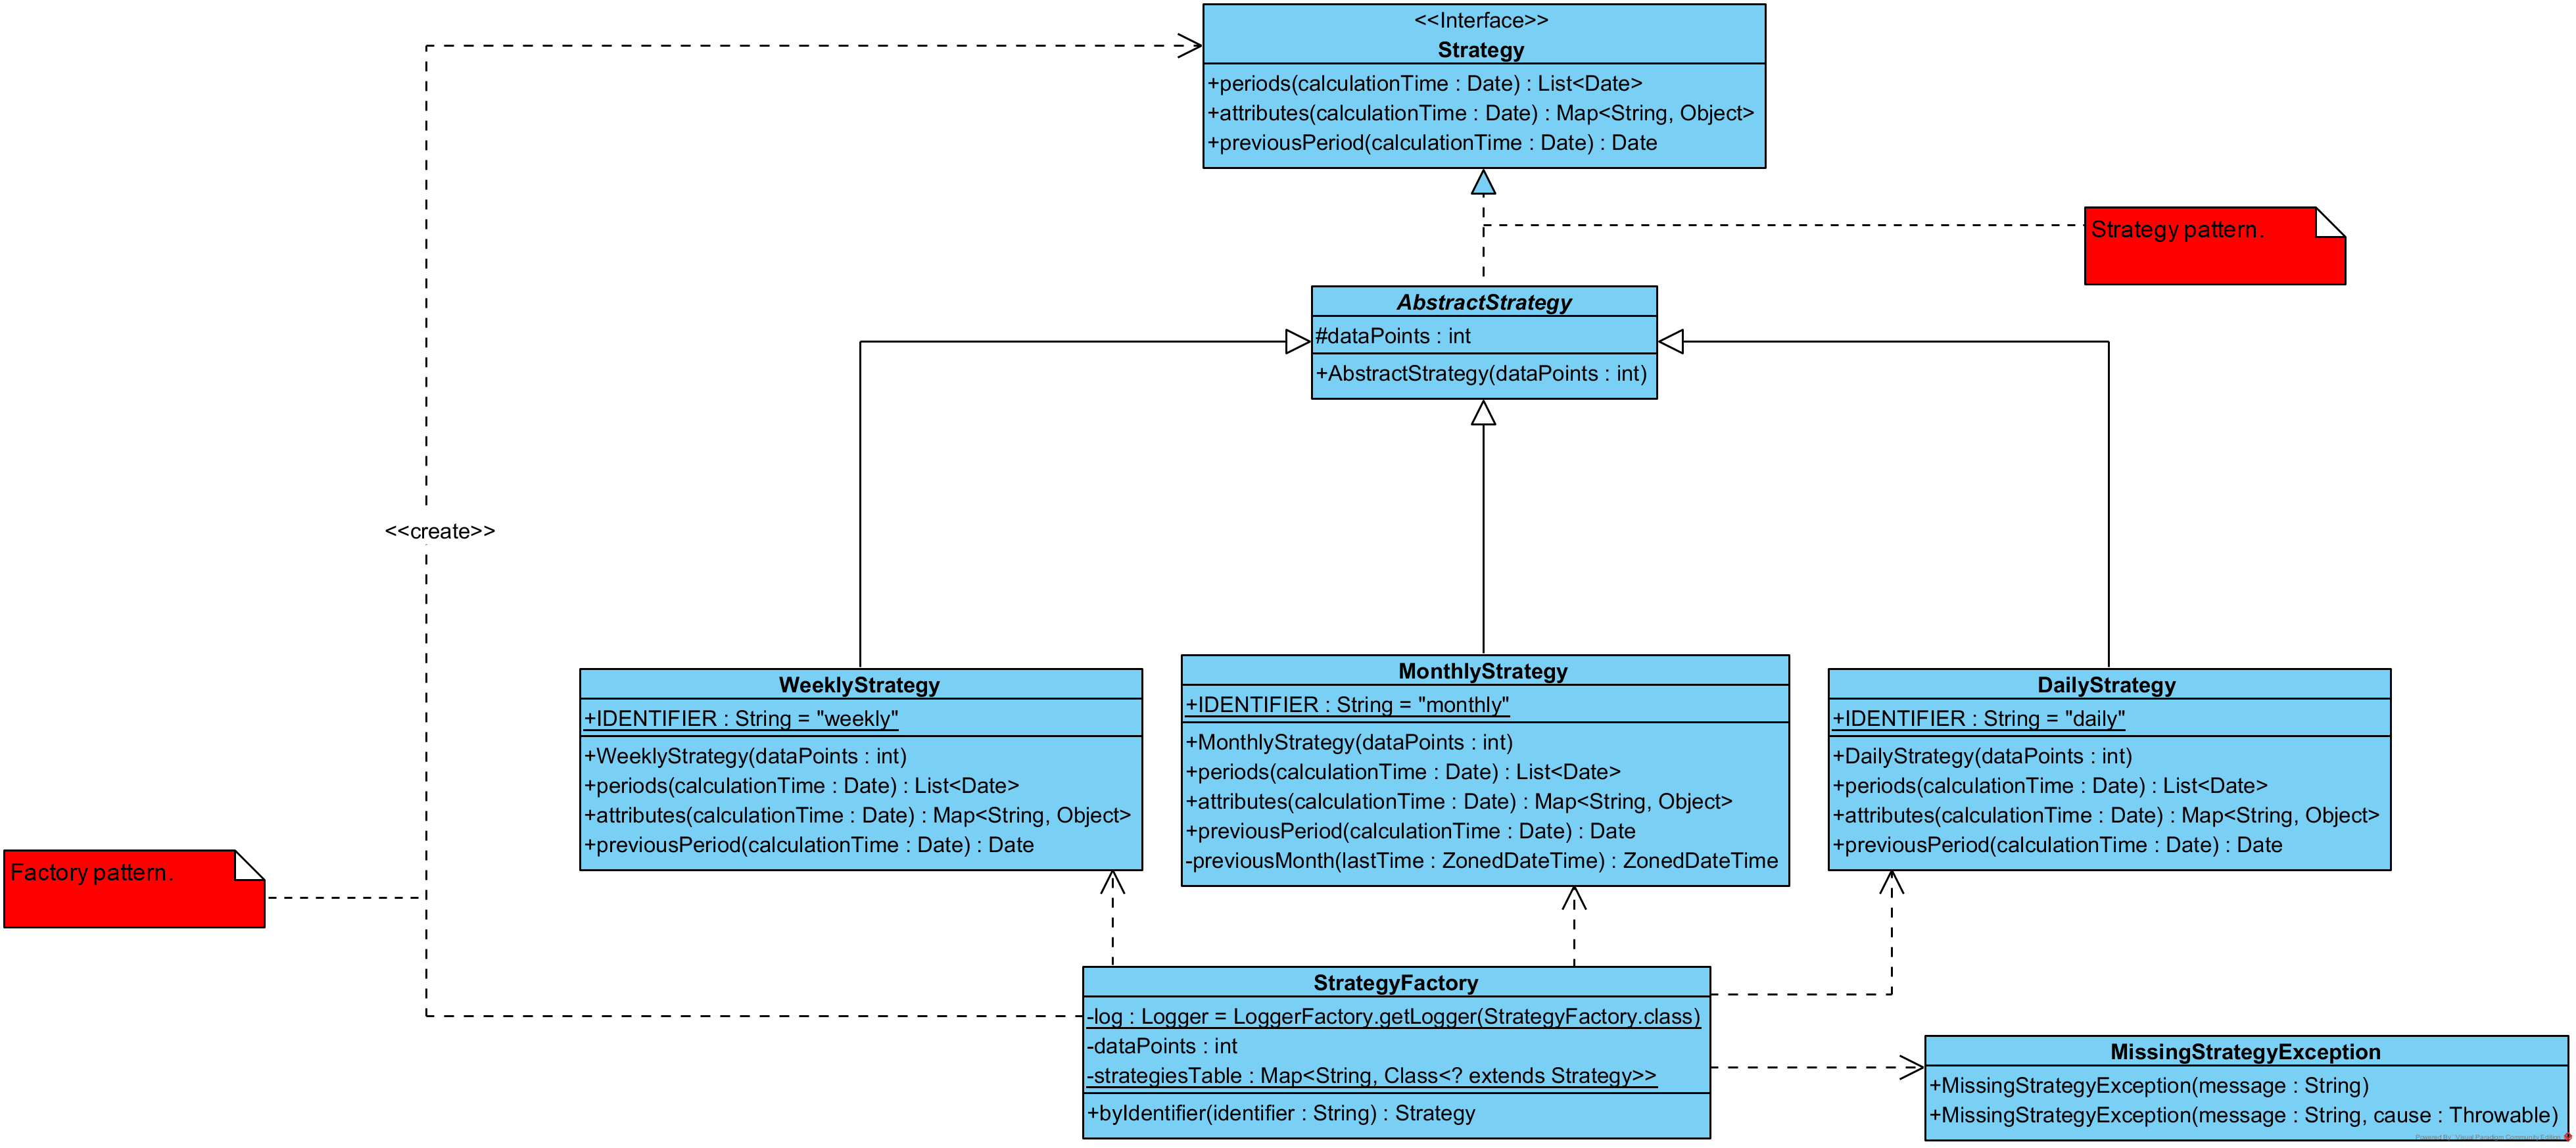
\includegraphics[width=\textwidth]{./img/DiagrammiClasse/Strategies.png}
            \caption[Diagramma del package strategies]{Diagramma del package strategies}
       	\end{figure}
		
		\paragraph*{Descrizione}
			Questo package contiene le classi che vanno a descrivere la strategia con cui si vanno a 
			calcolare le baseline.\\
			Il procedimento per aggiungerne di nuove è descritto in §\ref{newstrategy}.
		
		\paragraph*{Classi}
		
			\begin{itemize}
				\item \textbf{AbstractStrategy:} classe astratta di una strategia che gestisce le proprietà 
					di default;
				\item \textbf{DailyStrategy:} classe per calcolare baseline su base giornaliera;
				\item \textbf{MissingStrategyException:} eccezione lanciata quando non è possibile definire 
					una strategia a causa di parametri in input non validi;
				\item \textbf{MonthlyStrategy:} classe per calcolare baseline su base mensile;
				\item \textbf{Strategy:} interfaccia di una strategia per il calcolo di una baseline;
				\item \textbf{StrategyFactory:} classe che  permette di costruire una strategia in base 
					ad una configurazione scelta;
				\item \textbf{WeeklyStrategy:} classe per calcolare baseline su base settimanale.
			\end{itemize}

\newpage
		
	\subsubsection{templators}
		
		\paragraph*{Descrizione}
			In questo package sono contenute classi utili per creare date e operatori.
		
		\paragraph*{Classi}
			\begin{itemize}
				\item \textbf{IndexTemplator:} classe utilizzata per gestire i nomi degli indici;
				\item \textbf{OperandTemplator:} classe utilizzata per gestire gli operandi
					nelle operazioni.
			\end{itemize}
		
	\subsubsection{utils}
		
		\paragraph*{Descrizione}
			Questo package contiene classi utilizzate principalmente come utilità.
		
		\paragraph*{Classi}
			\begin{itemize}
				\item \textbf{Debouncer:} semplice implementazione di un debouncer.
			\end{itemize}					
		